%%%%%%%%%%%%%%%%%%%%%%%%%%%%%%%%%%%%%%%%%%%%%%%%%%%%%%%%%%%%%%%%%%%%
%% I, the copyright holder of this work, release this work into the
%% public domain. This applies worldwide. In some countries this may
%% not be legally possible; if so: I grant anyone the right to use
%% this work for any purpose, without any conditions, unless such
%% conditions are required by law.
%%%%%%%%%%%%%%%%%%%%%%%%%%%%%%%%%%%%%%%%%%%%%%%%%%%%%%%%%%%%%%%%%%%%

\documentclass[
  digital,     %% The `digital` option enables the default options for the
               %% digital version of a document. Replace with `printed`
               %% to enable the default options for the printed version
               %% of a document.
%%  color,       %% Uncomment these lines (by removing the %% at the
%%               %% beginning) to use color in the printed version of your
%%               %% document
  oneside,     %% The `oneside` option enables one-sided typesetting,
               %% which is preferred if you are only going to submit a
               %% digital version of your thesis. Replace with `twoside`
               %% for double-sided typesetting if you are planning to
               %% also print your thesis. For double-sided typesetting,
               %% use at least 120 g/m² paper to prevent show-through.
  nosansbold,  %% The `nosansbold` option prevents the use of the
               %% sans-serif type face for bold text. Replace with
               %% `sansbold` to use sans-serif type face for bold text.
  nocolorbold, %% The `nocolorbold` option disables the usage of the
               %% blue color for bold text, instead using black. Replace
               %% with `colorbold` to use blue for bold text.
  lof,         %% The `lof` option prints the List of Figures. Replace
               %% with `nolof` to hide the List of Figures.
  lot,         %% The `lot` option prints the List of Tables. Replace
               %% with `nolot` to hide the List of Tables.
]{fithesis4}
%% The following section sets up the locales used in the thesis.
\usepackage[resetfonts]{cmap} %% We need to load the T2A font encoding
\usepackage[T1,T2A]{fontenc}  %% to use the Cyrillic fonts with Russian texts.
\usepackage[
  main=english, %% By using `czech` or `slovak` as the main locale
                %% instead of `english`, you can typeset the thesis
                %% in either Czech or Slovak, respectively.
  english, german, czech, slovak %% The additional keys allow
]{babel}        %% foreign texts to be typeset as follows:
%%
%%   \begin{otherlanguage}{german}  ... \end{otherlanguage}
%%   \begin{otherlanguage}{czech}   ... \end{otherlanguage}
%%   \begin{otherlanguage}{slovak}  ... \end{otherlanguage}
%%
%%
%% The following section sets up the metadata of the thesis.
\thesissetup{
    date        = \the\year/\the\month/\the\day,
    university  = mu,
    faculty     = fi,
    type        = bc,
    department  ={Department of Computer Systems and Communications},
    author      = Jindřich Halabala,
    gender      = m,
    advisor     = {RNDr. Ondřej Krajíček},
    title       = {Experimenting with web-page structural analysis using Deep Reinforcement Learning},
    TeXtitle    = {Experimenting with web-page structural analysis using Deep Reinforcement Learning},
    keywords    = {deep reinforcement learning, user interface element detection, object detection, computer vision, PPO, YOLO},
    TeXkeywords = {deep reinforcement learning, user interface element detection, object detection, computer vision, PPO, YOLO},
    abstract    = {%

    This thesis investigates the feasibility of using deep reinforcement learning for detecting graphical user interface elements in web application screenshots. To do so, ten reinforcement learning environments of increasing complexity are developed, and agents are trained in each using a variety of reward functions, network architectures, and hyperparameters until an agent capable of solving each environment is achieved. The performance of the resulting model is then compared with two prototypes developed using traditional approaches: traditional computer vision and deep supervised learning. The thesis concludes that, while training a model purely through reinforcement learning is feasible, it does not offer significant advantages for this particular problem.
    },
    thanks      = {
    I would like to express my sincere gratitude to my supervisor, RNDr. Ondřej Krajíček, for his invaluable guidance, insightful feedback, and unwavering support throughout the development of this thesis. His mentorship was instrumental in shaping the direction and quality of my work.

    My heartfelt thanks also go to the entire YSoft AIVA team for fostering such a supportive and collaborative environment. Without them, I would not have the opportunity to investigate such an interesting topic.
    
    Finally, I am deeply grateful to my family and friends for their continuous encouragement and understanding. Their support helped me stay motivated and focused, especially during the most challenging moments of this journey.

    },
    bib         = example.bib,
    %% Remove the following line to use the JVS 2018 faculty logo.
    facultyLogo = fithesis-fi,
}
\usepackage{makeidx}      %% The `makeidx` package contains
\makeindex                %% helper commands for index typesetting.
%% These additional packages are used within the document:
\usepackage{paralist} %% Compact list environments
\usepackage{amsmath}  %% Mathematics
\usepackage{amsthm}
\usepackage{amsfonts}
\usepackage{url}      %% Hyperlinks
\usepackage{markdown} %% Lightweight markup
\usepackage{listings} %% Source code highlighting
\usepackage{svg}      %% SVG figures
\lstset{
  basicstyle      = \ttfamily,
  identifierstyle = \color{black},
  keywordstyle    = \color{blue},
  keywordstyle    = {[2]\color{cyan}},
  keywordstyle    = {[3]\color{olive}},
  stringstyle     = \color{teal},
  commentstyle    = \itshape\color{magenta},
  breaklines      = true,
}
\usepackage{floatrow} %% Putting captions above tables
\floatsetup[table]{capposition=top}
\usepackage[babel]{csquotes} %% Context-sensitive quotation marks
\begin{document}
%% The \chapter* command can be used to produce unnumbered chapters:
\chapter*{Introduction}
%% Unlike \chapter, \chapter* does not update the headings and does not
%% enter the chapter to the table of contents. I we want correct
%% headings and a table of contents entry, we must add them manually:
\markright{\textsc{Introduction}}
\addcontentsline{toc}{chapter}{Introduction}

Certain graphical user interface (UI) testing tools, such as YSoft AIVA, interact with applications solely based on visual information. In order to achieve this, they must reliably detect and localize interface elements in the captured image to infer the UI's hierarchical structure. This process is typically carried out using traditional computer vision algorithms or deep neural networks trained via supervised learning. The main focus is on finding the exact borders of the elements rather than, for example, classifying what types of elements are present.

This thesis investigates the experimental use of reinforcement learning (RL) algorithms for detecting user interface elements. First, a series of simulated environments with increasing complexity is created to model the problem. Next, agents are trained in these environments using various parameters and reward functions until they successfully learn to detect and localize visual elements, ranging from basic shapes to complete user interface components. This process results in an agent capable of accurately locating UI elements. Finally, the resulting approach is compared with traditional methods.

The thesis concludes that while training an agent for UI element detection purely by RL is possible, it does not bring any sizable benefits over the currently used techniques, while being less accurate and harder to train.

The thesis is organized into five chapters. The first chapter provides a detailed overview of the problem, existing solutions, their limitations, and the rationale for using RL. The second chapter outlines the theoretical and mathematical foundations of RL. The third chapter discusses the libraries and tools used for agent development and training. Next, the fourth chapter presents the design of simulated environments, the experiments that were conducted, and the challenges encountered. Finally, in the fifth chapter, the proposed approach is compared with traditional methods.

\chapter{User interface element detection}

YSoft AIVA\footnote{\url{https://www.ysoft.com/aiva}} is a tool for automated end-to-end testing of web applications. Unlike most competing tools, AIVA does not interact with the web page's Document Object Model (DOM). Instead, it relies entirely on visual information. This approach resembles black-box testing, as it mirrors how a real user interacts with the application, and enhances robustness in scenarios, such as when XPaths change due to newly added components. However, it introduces significant challenges, as all relevant information must be extracted from images rather than a structured markup language.

A crucial aspect of data extraction is identifying the location, size, and hierarchical relationships of all key interactive elements on a web page (e.g., buttons, icons, text fields). If performed correctly, it allows AIVA to reconstruct the DOM and localize correct elements during test execution.

This task can be addressed through either object detection or segmentation, as most objects on a web page are rectangular. However, due to the hierarchical nature of the DOM, detection is the more intuitive choice. A single pixel can belong to multiple overlapping elements, which complicates segmentation. That said, the detected information can be converted into a segmentation map if needed. This relationship is illustrated in Figure~\ref{fig:example-result}.

\begin{figure}
    \centering
    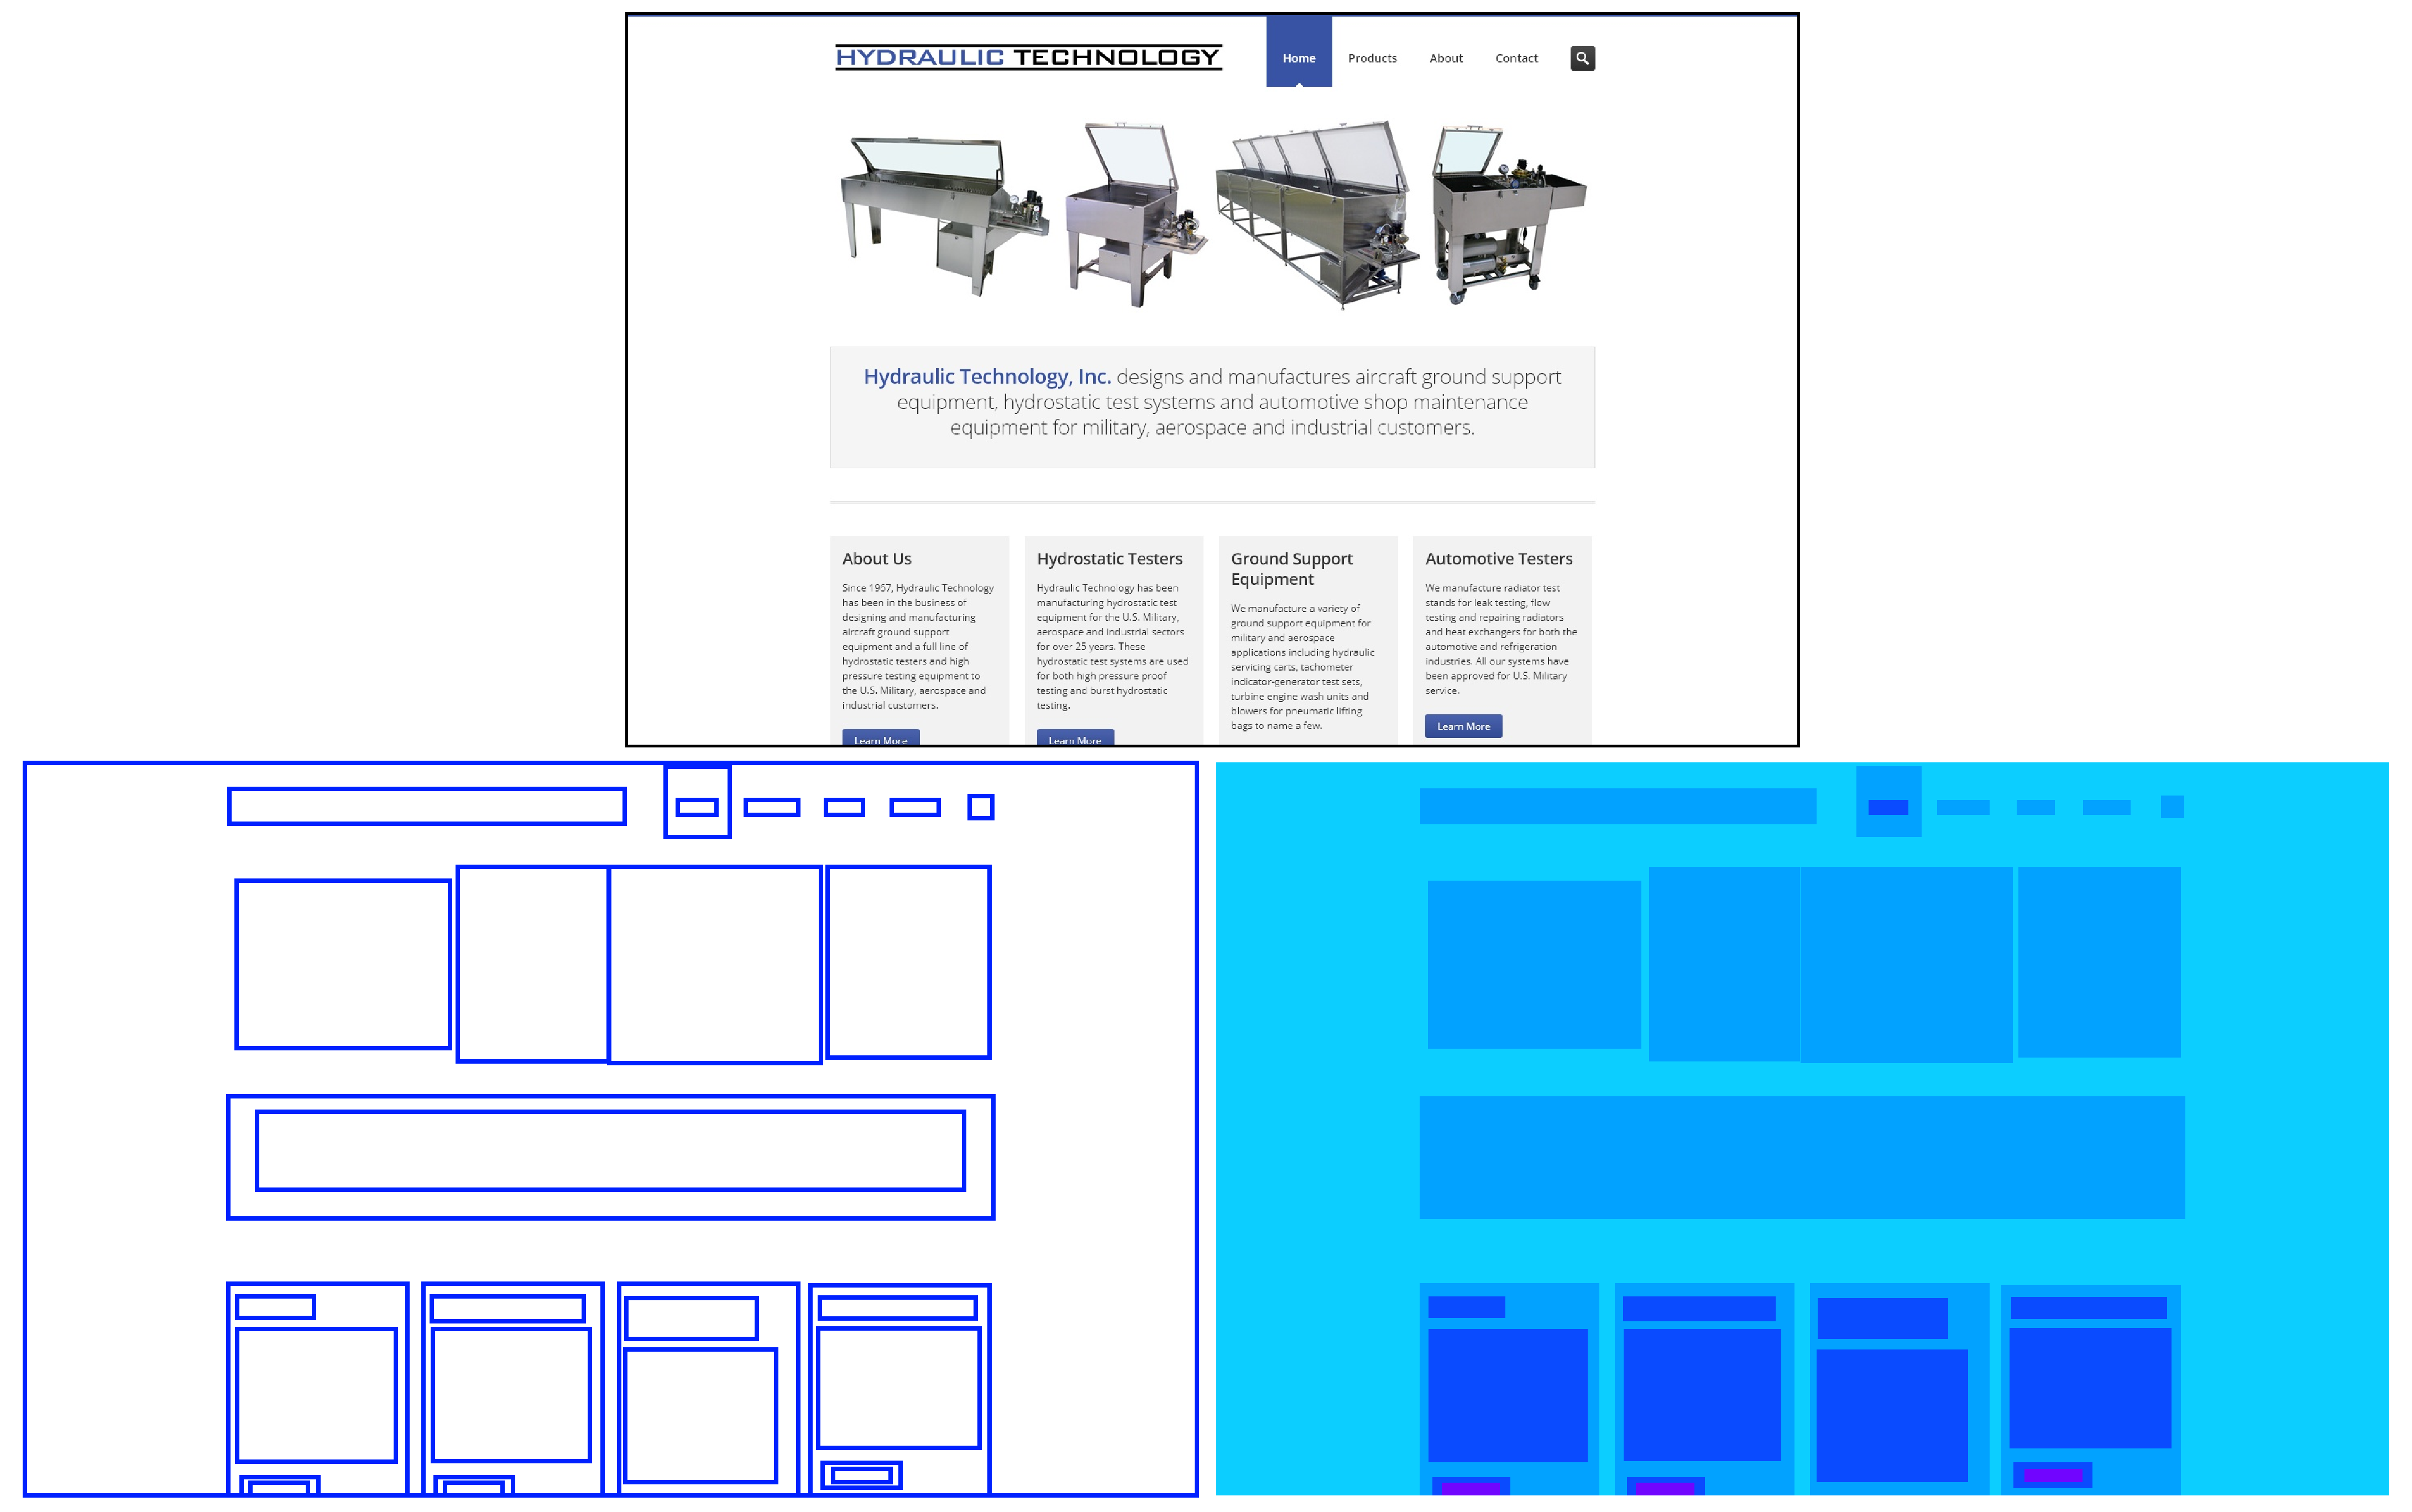
\includegraphics[width=0.7\linewidth]{diagrams/result_example.pdf}
    \caption{An example of a processed web page. The top image is the original screenshot, the middle image shows bounding boxes of detection, and the bottom image shows the same information but as a segmentation map. The original screenshot comes from~\cite{aydos2020}.}
    \label{fig:example-result}
\end{figure}

Graphical user interface (GUI) object detection is usually performed using traditional computer vision (CV) or using deep learning-based object detection models such as R-CNNs or YOLO. A combination is also possible, for example, using a deep learning (DL) model for text and image detection and CV for the rest~\cite{ODforGUI_CV_DL_or_both}. This chapter looks at both approaches, some existing solutions based upon them, and the challenges they present. Finally, a third approach that could solve these problems is proposed based on deep reinforcement learning.

\section{Traditional computer vision-based solutions}
\label{sec:traditionalCV}

In this thesis, the term \enquote{traditional computer vision} refers to digital image processing algorithms that do not use machine learning but operate directly on pixel data. Traditional CV is challenging to use for object detection in photographs due to noise and unclear edges. However, it is well-suited for processing user interfaces. Screenshots typically lack noise (aside from occasional compression artifacts) and contain clearly defined edges

A common approach involves applying an edge detection method (e.g., Canny or Sobel), followed by post-processing steps to make the edges cleaner (e.g., morphological operations, filtering of small edges), and finally, detecting contours in the binary image. The resulting edge data can be combined with outputs from an optical character recognition (OCR) model and further processed to merge similar elements and filter out small elements that are likely just noise. This process is employed in algorithms such as REMAUI~\cite{remaui} (a tool for reverse engineering of mobile application GUIs), UISeg~\cite{uiseg} (user interface segmentation algorithm), and also in the current implementation of AIVA's element detection procedure.

Template matching represents another localization approach, though it lacks flexibility. It works reliably for highly standardized elements (e.g., checkboxes or buttons in desktop applications with a fixed GUI style). However, it is ineffective for mobile or web applications where GUI components vary widely in design~\cite{ODforGUI_CV_DL_or_both}.

Despite recent advances in deep learning, traditional CV continues to offer several advantages. It can be much more efficient and straightforward to understand, making it easier to modify and debug. Each step of the algorithm can be observed, facilitating debugging and parameter adjustment. These sorts of modifications are difficult to achieve with DL. Another significant benefit is the reduced dependency on large training datasets, which require a lot of manual labor to create. Furthermore, this reliance increases the risk of obsolescence, as DL-based models may not generalize well to evolving GUI design trends~\cite{DLvsTCV}.

\section{Supervised deep learning-based solutions}
Over the past decade, state-of-the-art object detection algorithms have relied almost exclusively on deep neural networks incorporating convolutional layers. Two of the most prominent model families are Region-based Convolutional Neural Networks (R-CNNs) and You Only Look Once (YOLO). Generally, R-CNNs offer higher accuracy, while YOLO provides better speed, though performance varies by model and use case~\cite{ObjectDetectionHistorySurvey}.

One example of a deep learning-based GUI element detection algorithm is OmniParser\footnote{\url{https://microsoft.github.io/OmniParser/}}, a fine-tuned YOLOv8 model for parsing and labeling GUIs. It was created to enhance the performance of large multi-modal agents like GPT-4V~\cite{OmniParser}. Daneshvar et al.~\cite{GUI_YOLO_comparison} evaluated various YOLO architectures for GUI element detection, achieving promising results. During its earlier use for testing physical touchscreen devices, AIVA employed a model based on the Single Shot Detection (SSD) architecture~\cite{Horak2020thesis}.

A major advantage of DL-based approaches lies in their ability to automatically learn complex patterns from data, without requiring explicit programming or manual domain-specific tuning. However, as stated in the previous section, this reliance on a dataset is also one of the main drawbacks. Moreover, both training and inference phases typically require significantly more computational resources than traditional CV algorithms~\cite{DLvsTCV}.

\section{Object detection with reinforcement learning}

The previous two sections highlight two significant challenges. Traditional CV is insufficient for more complex images, while supervised DL methods require access to large, high-quality datasets\footnote{By \enquote{high-quality} I mean a dataset that is large, has accurate annotations, and includes larger enclosing elements. More in Subsection~\ref{subsec:dataset}.}. A combination of both could, in theory, eliminate or at least mitigate these drawbacks. One possible solution involves creating a function that evaluates bounding box prediction quality based on traditional CV techniques. This function could then serve as a supervisory signal for training a deep learning model, thus eliminating the need for manually labeled ground-truth bounding boxes. Instead, only images of web applications would be required, which are significantly easier to obtain.

Supervised learning models are not applicable if we only have a numerical score for predictions rather than ground truth labels. Instead, we can use a reinforcement learning model that learns from evaluative feedback (more details on RL in Chapter~\ref{ch:dlr}).

To the best of my knowledge, no author has investigated multi-object detection using reinforcement learning. Nonetheless, prior studies have examined its use for single-object detection in photographs~\cite{iterative_od_with_rl, hierarchical_od_with_drl} and for region proposal in multi-object detection~\cite{drl_rpn}. They all use ground-truth labels for learning.

\chapter{Deep reinforcement learning}
\label{ch:dlr}

The theory behind reinforcement learning is essential for understanding the terminology and decisions presented in the following chapters. This chapter provides the necessary background to understand the remainder of this thesis. Note that this is a brief, non-exhaustive introduction covering only the most important algorithms and definitions.

Unless stated otherwise, the notation and information used in this chapter are adopted from \textit{Grokking Deep Reinforcement Learning} by Miguel Morales~\cite{GDRL}.

\section{Machine learning}
Machine learning (ML) is the study of algorithms that allow computers to learn from data without explicit programming. It can be split into three main categories: supervised learning, unsupervised learning, and reinforcement learning\footnote{Other categories, such as semi-supervised or self-supervised learning, are also recognized, but these are generally modifications or combinations of the three primary categories.}~\cite{IB031}.

In supervised learning (SL), the goal is to make predictions based on labeled data available during training, such as in classification or regression tasks. In unsupervised learning (UL), no correct labels are known, so it is more about finding patterns in the provided data. This approach can be used to, for example, separate the data into groups (clustering) or to generate new, similar data using models such as autoencoders or generative adversarial networks~\cite{IB031, PV021}.

Similar to SL, reinforcement learning involves learning a mapping from inputs to outputs, but differs fundamentally in the type of feedback provided. Unlike in SL, where the correct labels are provided for training purposes, RL relies only on the feedback from a reward function. This function evaluates the agent's decisions based on their outcomes, by providing scalar feedback that reflects the quality of the chosen actions. The agent aims to learn to make decisions that maximize this reward through trial and error. RL is ideal for decision-making, especially in environments where the optimal strategy is unknown or difficult to obtain.

\section{Reinforcement learning}
Reinforcement learning problems consist of two interacting entities: the agent and the environment. The agent is the algorithm taught to make decisions. The environment comprises everything external to the agent. For example, in a driving task, the environment includes other vehicles, road conditions, pedestrians, and the controlled car itself.

The typical interaction between agent and environment in RL follows a cycle, as illustrated in Figure~\ref{fig:rl-cycle}. In the beginning, the environment is in some initial state. The agent observes the state (although in many cases, it may only have access to a partial observation of the full state) and chooses an action it thinks is the best. The environment receives and reacts to this choice, changing its inner state. The agent observes this new state and gets rewarded based on the chosen action. The agent can then update its behavior based on this feedback. Then, it again chooses an action, and the cycle repeats.

\begin{figure}
    \centering
    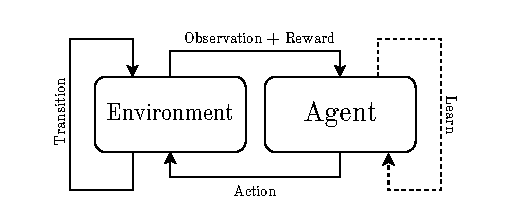
\includegraphics[width=1\linewidth]{diagrams/rl_cycle.pdf}
    \caption{The reinforcement learning cycle}
    \label{fig:rl-cycle}
\end{figure}

A single iteration of this cycle is referred to as a time step, and it generates an experience -- a tuple of the original state $s$, the action taken $a$, the reward given $r$, and the new state $s'$. Depending on the task, the cycle may continue indefinitely or terminate once the environment reaches a designated terminal state. For example, in a chess game, the end is defined as winning, losing, or a draw. Such tasks are called episodic, with all experiences from the initial to the terminal state forming an episode. If there is no well-defined end, the task is referred to as continuous.

The reward function may be dense, sparse, or lie somewhere in between. A dense reward function awards the agent a non-zero reward in each iteration of the RL cycle. A sparse reward function only gives a non-zero reward when the environment transitions into a terminal state. While dense reward functions are generally easier to learn from, in some cases, they can be challenging to implement. In the chess example, we know that losing is negative and winning is positive, but judging a single move is problematic unless we know the optimal strategy.

Reinforcement learning is challenging due to the sequential, evaluative, and sampled nature of the feedback.

The sequentiality comes from the fact that most tasks span multiple time steps. The consequences of an action might not be immediately apparent. When an episode ends with a very negative result, it can be difficult to determine which of the preceding actions is the cause, as it is often not the last action taken.

Evaluative feedback refers to the reward being provided as a scalar value. Without additional context, it is impossible to know if the received reward was the best possible and if we should thus repeat the decision in similar states or whether it was terrible and should be avoided in the future. This issue leads to the need for exploration discussed in Section~\ref{sec:explor-exploit}.

The agent can only learn from the states it has visited and the actions it has taken, thus the feedback it gets is sampled. In many real-life RL problems, there are so many states that trying every combination of state and action is impossible. This challenge also exists in supervised learning, as the dataset will never contain all the data the model might encounter. However, in reinforcement learning, this problem is even worse as the agent must collect all the data on its own.

\section{Markov decision process}
In order to define RL and its objective, it is first necessary to define the environment. There are multiple ways to do so, but the most common representation is a Markov decision process (MDP). An MDP is defined as a tuple $(S, A, p, r)$.

$S$ is the state space, a set of all possible environment states. It can contain both discrete and continuous values. At each time step $t$, the MDP is in a state $s_t\in S$.

$A$ is the action space, a set of all possible actions an agent can perform within the MDP. It may also be discrete, continuous, or a combination of both. At each time step $t$, the agent chooses an action $a_t\in A$ based on the observed state $s_t$.

$p$ is the probabilistic transition function $p\colon S \times A \to \mathcal{D}(S)$. For a given state $s\in S$ and a given action $a\in A$, it returns a probability distribution $\mathcal{D}(S)$ over the states $s'\in S$. It specifies the probability of the MDP transitioning from the state $s$ to a state $s'$ given that an action $a$ was selected. Formally, it is defined as:
\begin{equation}
p(s' \mid s,a)=P(S_t=s'\mid S_{t-1}=s,A_{t-1}=a)    
\end{equation}
The sum of all transition probabilities for each state-action pair must equal one:
\begin{equation}
\sum_{s'\in S} p(s'\mid s,a)=1, \forall s \in S, \forall a \in A
\end{equation}

If the environment does not allow for some action $a^{\times}$ to be performed in a state $s$, we define a degenerate transition distribution for that state-action pair:
\begin{equation}
    p(s'\mid s, a^{\times}) =\begin{cases}1 & s' = s\\0 & \text{otherwise} \end{cases} 
\end{equation}

Lastly, $r$ is the reward function. Depending on the use case, it can be defined either as $r\colon S \times A \to \mathbb{R}$ -- the expected reward for choosing an action $a$ in a state $s$~\cite{PA230}:
\begin{equation}
r(s,a)= \mathbb{E} [R_t\mid S_{t-1}=s, A_{t-1}=a]
\end{equation}
or as $r\colon S\times A \times S \to \mathbb{R}$ -- the expected reward for choosing an action $a$ in a state $s$ given we transition into a state $s'$:
\begin{equation}
r(s, a, s')= \mathbb{E} [R_t\mid S_{t-1}=s, A_{t-1}=a, S_t=s']
\end{equation}

The initial state distribution is typically defined over a subset of states $S^i \subseteq S$. When an MDP is initialized, the initial state is chosen from this subset using a probability distribution $\mathcal{I}$ over these states.

Similarly, a set of all terminal states may be defined. The MDP terminates when it transitions into one of the terminal states. Alternatively, terminal states can be modeled as absorbing states, eliminating the need for explicit definition. This involves defining the transition function such that any action taken in a terminal state leads back to that same state with a probability of one, and ensuring the reward for such transitions is zero.

Simple Markov decision processes can be visualized as diagrams, as illustrated in Figure~\ref{fig:mdp}.

\begin{figure}
    \centering
    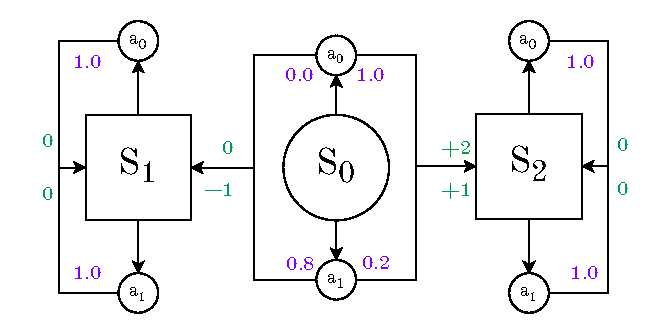
\includegraphics[width=1\linewidth]{diagrams/mdp.pdf}
    \caption{Graphical representation of a Markov decision process. Squares depict terminal states. Transition probabilities (purple) and rewards (green) are indicated.}
    \label{fig:mdp}
\end{figure}

\subsection{Markov property}
\label{subsec:markov_property}
The probabilistic transition function $p$ only takes the current state and action as inputs. Notably, it does not take into account the history of past states or actions. The probability of transitioning to state $s'$ after taking action $a$ in state $s$ is independent of the sequence of prior states and actions that led to $s$. This memorylessness of MDPs is known as the Markov property. This property is important to remember during environment implementation, as many RL algorithms operate under the assumption that it is satisfied. It can be formally defined as
\begin{equation}
P(S_{t+1}\mid S_t,A_t)=P(S_{t+1}\mid S_t,A_t,S_{t-1},A_{t-1}, \dotsc)
\end{equation}
An example of an environment that violates the Markov property is the game Pong\footnote{\url{https://en.wikipedia.org/wiki/Pong}}, where the state is only the current frame. A single frame does not provide sufficient information to determine the ball’s direction or speed after the next action. Thus, the history of the past states is required. This issue can be addressed by explicitly including the ball’s position, speed, and direction in the state representation (or using other techniques such as frame-stacking, where multiple preceding frames are included in the observation).

\subsection{Partially observable MDPs}
Standard MDPs may be insufficient for accurately modeling real-world environments; however, various extensions have been proposed to address these limitations. In RL, we often encounter partially observable MDPs (POMDPs) where the agent does not have access to the true state but only an observation of it. POMDPs further define the observation space $\mathcal{O}$ and a state-observation mapping function $\epsilon \colon S \to \mathcal{D}(\mathcal{O})$.

\section{Policy}
With the environment formally defined as an MDP, the agent can also be defined. The agent can be viewed as an entity that, upon receiving a state $s$ (or an observation of it), selects an action $a$, which results in a reward $r$ and a transition to a new state $s'$. As mentioned, the tuple $(s, a, r, s')$ is referred to as an experience. The entire sequence of these experiences is called a trajectory $\tau$. Since the final state of one experience is the initial state of the next, the trajectory can be simplified as follows: $s_0,a_0,r_1,s_1,a_1,r_2,\dotsc \in (S\times A \times \mathbb{R})^{*}$. Note that, depending on the type of task and definition of the terminal states, the trajectory can be infinitely long. A history is then some finite prefix of a trajectory ending in a state: $s_0,a_0,r_1,s_1,a_1,r_2,\dotsc, a_{t-1},r_t,s_t\in (S\times A \times \mathbb{R})^{*}\times S$.
The agent's behavior is governed by a policy. A policy $\pi$ is a function $\pi\colon (S\times A \times \mathbb{R})^{*}\times S \to \mathcal{D}(A)$, which returns a probability distribution over the action space based on the history up to that point~\cite{PA230}.

If the environment satisfies the Markov property, the policy definition can be simplified to just $\pi\colon S \to \mathcal{D}(A)$ because, in that case, the environment is memoryless, and thus, it does not matter how it ended up in the state $s_t$. Thanks to this, the agent (and its underlying policy) can also be memoryless. Note that this is only true if the agent receives the entire state, so this simplification can not be applied to POMDPs (two different states might produce the same observation, and the history might be helpful to differentiate between them).

We can further simplify the policy by making it deterministic -- instead of returning a probability distribution $\mathcal{D}(A)$, it returns a single action $a$. Such a policy can be defined as just $\pi\colon S\to A$.

\section{The goal of RL}
\label{sec:goal}
With the environment (MDP) and the agent (policy) formally defined, we can now define the objective of reinforcement learning. The objective is to find an optimal policy $\pi^*$ that maximizes the expected discounted cumulative reward, commonly referred to as the discounted return. The cumulative reward (or return) of a trajectory $\tau$ is the sum of all received rewards:
\begin{equation}
G(\tau) = r_1+r_2+r_3+\dotsb = \sum_{i=1}^{\infty} r_i
\end{equation}
The discounted return is obtained by applying an exponential decay to future rewards using a discount factor $\gamma \in [0,1]$. Discounting serves two purposes. First, since trajectories can be infinite, a policy that enters a reward-generating cycle (even with small rewards) could result in an infinite return. Second, it encourages policies to achieve rewards sooner, as earlier rewards are less heavily discounted. The discounted return $G$ on a trajectory $\tau$ with discount factor $\gamma$ is defined as:
\begin{equation}
G(\tau)=r_1+\gamma \cdot r_2+ \gamma^2 \cdot r_3+\dotsb = \sum_{i=1}^{\infty} \gamma^{i-1}\cdot r_{i}
\end{equation}
Finally, we consider the expected discounted return. Since environments are often stochastic, initial states may vary, and the identical state-action pair may lead to different transitions each time. As a result, even a deterministic policy can produce different trajectories in the same MDP, each yielding potentially different returns. Thus, it is important to find such a policy that will, on average, have the highest discounted return, rather than optimizing for any particular instance.

\section{Value functions}

For a given policy $\pi$, we define value functions that measure its performance within a specific environment. These functions are useful for comparing policies and play a central role in many learning algorithms (see Subsection~\ref{subsec:value-based-methods}).

\subsection{State-value function}
\label{subsec:state_value_func}
The state-value function $v_\pi\colon S\to \mathbb{R}$ (often referred to as just the value function) gives the expected return of policy $\pi$ when starting in a state $s$.
\begin{equation}
v_\pi(s) = \mathbb{E}_\pi [G_t\mid S_t=s]
\end{equation}

If we have access to the underlying MDP, we can calculate the state-value function directly using the Bellman equation:

\begin{equation}
v_\pi(s) = \sum_a \pi(a\mid s) \cdot \sum_{s',r} p(s',r\mid s,a)\cdot[r+\gamma v_\pi(s')], \forall s \in S
\end{equation}

Due to the recursive nature of this formula, it would be difficult to calculate directly, so in practice, an iterative algorithm that uses an already existing approximation for the next state is used. When the environment's dynamics are unknown, sample-based methods such as Monte Carlo and temporal difference are employed to approximate value functions through interaction.

\subsection{Action-value function}

While the state-value function indicates the quality of a state, it is of little help when choosing an action unless the agent also knows the transition function. The action-value function $q_\pi\colon S \times A \to \mathbb{R}$ provides the expected return when taking an action $a$ in a state $s$ and following policy $\pi$ from there.

\begin{equation}
q_\pi(s,a) = \mathbb{E}_\pi [G_t\mid S_t=s,A_t=a]
\end{equation}

Action-value functions are particularly useful for improving policies and form the foundation of algorithms such as Q-learning and Deep Q-Networks (DQN).

\subsection{Action-advantage function}

Lastly, the advantage function $a_\pi$ quantifies how much better or worse taking a specific action $a$ in a state $s$ is, compared to the expected performance of following policy $\pi$:

\begin{equation}
a_\pi(s,a) = q_\pi(s,a)-v_\pi(s)
\end{equation}

In practice, especially when using neural networks as function approximators, it is common to estimate the state-value and advantage functions separately and then combine them to produce the action-value function. This approach is known as the dueling network architecture and was introduced in~\cite{dueling_arch}.

\section{Exploration-exploitation tradeoff}
\label{sec:explor-exploit}
As mentioned in Subsection~\ref{subsec:state_value_func}, many RL algorithms rely on approximating a value function using an iterative algorithm and then use this information to improve the policy. The agent must interact with the environment repeatedly to collect experiences and improve the approximation. To create the best approximation, it would be ideal to run the policy from every possible state and evaluate every possible action, ideally many times, to account for randomness. This is clearly infeasible for environments with more than a few thousand states, and it is impossible for environments with continuous state or action spaces.

Since exhaustive exploration is infeasible, RL algorithms must balance two competing objectives: discovering new strategies (exploration) and leveraging known good strategies (exploitation). This challenge is known as the exploration-exploitation tradeoff. Should we rather try new actions and risk spending time on unproductive paths (exploration), or stick to strategies that are already known to perform reasonably well (exploitation)?

The goal is to find the optimal policy while minimizing the number of time steps needed to do so. To manage this tradeoff effectively, various exploration strategies have been developed. Below are three commonly used approaches:

\begin{itemize}
    \item (Decaying) epsilon-greedy exploration strategy -- at each decision point, a random action is selected with probability $\varepsilon \in [0,1]$, otherwise, the action currently estimated to be the best is chosen. Typically, $\varepsilon$ decays over time to minimize exploration in the later stages of training.
    \item Upper confidence bound strategy -- when choosing which action to perform next, a bonus is added to the estimates with lower confidence (those that are less explored). The bonus is calculated as $c\sqrt{\frac{\ln{t}}{N_t(a)+1}}$ where $c$ is a constant describing the importance of this bonus, $t$ is the episode number and $N_t(a)$ is how many times the action $a$ was already chosen in this state (plus one to avoid division by zero).
    \item Softmax exploration strategy -- the probability of selecting an action is proportional to the exponentiated estimate of its action value. To get the probabilities, we pass the estimates through the softmax function, which will normalize them so that they are all between zero and one and their sum is equal to one. The softmax function is defined as $\sigma (v)_i = \frac{e^{v_i}}{\sum^{K}_{j=1}e^{v_j}}$ for the $i$-th value of a vector $v$ with $K$ elements. This strategy may not work well at the beginning when the estimates have high variance. To combat this issue, we divide the estimates by a decaying hyperparameter $\tau$ called temperature. This makes the differences in estimates less important at the beginning of the training.
\end{itemize}



\section{Reinforcement learning algorithms}
\label{sec:algos}

Over the last decade, numerous reinforcement learning algorithms have been proposed. The following subsections present the three main categories of reinforcement learning algorithms, along with selected examples. Exact descriptions of the individual algorithms are not provided, since they are not necessary for understanding the subsequent chapters.

\subsection{Value-based methods}
\label{subsec:value-based-methods}

The most straightforward approach to reinforcement learning is learning to approximate the action-value function (either directly or by computing it using the state-value and advantage-value functions) and then using a greedy policy that selects the best action based on these approximations.

In simple environments with small, discrete state and action spaces, each state-action combination estimate can be explicitly represented in a table. There are many different algorithms utilizing this principle (known as tabular algorithms). They differ in the way they calculate the approximations (temporal difference (TD), Monte Carlo (MC), $\lambda$-TD), whether they use the same model for the approximation and exploration (SARSA, Q-learning), and in their exploration strategies. Some more advanced algorithms approximate not only the Q function but also the underlying MDP to learn more efficiently (Dyna-Q).

While tabular algorithms perform well in simple environments, they become infeasible in more complex scenarios. Even for just a $100 \times 100$ pixel binary image state, $2^{10\,000} \approx 10^{3\,010}$ estimates would be necessary for each action.

In complex environments, deep learning techniques are employed to approximate value functions. The approximator is a neural network whose loss function is calculated as the difference between the approximations and actual values gathered during exploration. These methods often use a replay buffer -- a data structure that collects experience tuples from previous runs. During training, samples are drawn randomly from the buffer, which helps reduce bias caused by the experiences from one episode not being independent. These methods include algorithms such as Neural Fitted Q-iteration (NFQ), Deep Q-Learning (DQN), and Double DQN (DDQN).

\subsection{Policy-based methods}

While value-based methods create policies indirectly based on a value function, policy-based methods learn the policy directly by outputting a probability distribution over actions. Learning typically involves maximizing the probability of selecting actions with higher estimated advantages using gradient ascent.

Purely policy-based algorithms are rarely used nowadays, but they are an important part of the actor-critic architecture introduced in the following subsection. Policy-based algorithms include REINFORCE and Vanilla Policy Gradient (VPG).

\subsection{Actor-critic methods}

Actor-critic methods combine both value-based and policy-based methods into one. They consist of two components: the actor and the critic. The critic estimates the state-value function, while the actor represents the policy and selects actions. The critic learns just like the value-based methods by minimizing TD or MC errors. The actor then learns by maximizing the expected return based on the value estimations provided by the critic.

Actor-critic methods combine the strengths of both value-based and policy-based methods. They are more stable, more sample-efficient, and can deal with discrete and continuous action spaces. State-of-the-art actor-critic algorithms include Twin Delayed Deep Deterministic Policy Gradient (TD3), Soft Actor-Critic (SAC), and Proximal Policy Optimization (PPO).

\chapter{RL in practice}

The previous chapter provided a brief overview of the theory and terminology related to reinforcement learning. This chapter goes more into the practical part of RL, that is, the libraries used to implement environments and train agents in them. It provides the necessary context to understand the source code used in the experiments presented in this thesis.

As with most machine learning tasks, Python is one of the most popular programming languages for RL. Although AIVA is primarily implemented in .NET, using Python does not pose a limitation, as most machine learning libraries support model export to standard formats such as ONNX\footnote{\url{https://onnx.ai/}}. This enables agents trained in Python to be deployed natively in other programming environments, including .NET.

\section{Gymnasium}
\label{sec:gym}
Gymnasium\footnote{\url{https://gymnasium.farama.org/}} is a Python library that allows for easy creation of RL environments. It is an actively maintained fork of the Gym\footnote{\url{https://www.gymlibrary.dev/}} library developed by OpenAI. Its primary objective is to define a unified API for reinforcement learning environments. Additionally, it includes numerous wrappers that simplify tasks such as normalization, reward clipping, training monitoring, and parallel environment vectorization. The library also includes a wide range of predefined environments that can be used to evaluate new RL algorithms. The content of this section is based on the official Gymnasium documentation~\cite{gym-docs}.

In Gymnasium, an environment is implemented as a Python class that inherits from the \texttt{Env} base class. Within the class's initialization method, the observation and action space types must be specified. Gymnasium supports the following space types:

\begin{itemize}
    \item \texttt{Box} -- represents a fixed-shape $n$-dimensional tensor of numerical values. These values may be either bounded or unbounded. This type is commonly used to represent image observations or continuous action spaces.
    \item \texttt{Discrete} -- represents a space of finitely many integers. It is useful for representing discrete action spaces.
    \item \texttt{MultiBinary} -- represents a tensor of binary (boolean) values.
    \item \texttt{MultiDiscrete} -- represents a tensor of discrete values.
    \item \texttt{Text} -- a string composed of specified characters.
    \item Composite spaces -- fundamental space types can be combined using constructs such as \texttt{Dictionary}, \texttt{Tuple}, \texttt{Sequence} (of variable length), \texttt{Graph}, or \texttt{Union}.
\end{itemize}

The environment class is required to implement the following methods:

\begin{itemize}
    \item \texttt{reset} -- method called to begin a new episode. It resets the environment to an initial state and returns the initial observation and a dictionary with auxiliary information for debugging or other purposes. It takes a seed value as an optional parameter.
    \item \texttt{step} -- performs a single time step of the environment. Its only input is the action to be performed, which has to adhere to the type defined in the initialization method. It transitions the environment to a new state, and returns the new observation, the reward obtained from the action, a flag indicating whether the state is terminal, a flag indicating whether the episode was truncated (e.g., due to a time limit), and again, a dictionary with auxiliary information.
    \item \texttt{render} -- a method for getting the current state of the environment in a human-friendly format. Each environment can define multiple render modes, one of which can be selected during initialization. Common render formats include RGB frames, textual output, or sequences of RGB frames. This method can be called either manually by a user or by a monitoring wrapper of the environment.
    \item \texttt{close} -- a clean-up method. It should close render windows, end database connections, etc.
\end{itemize}

Once an environment is defined, it must be registered using the \texttt{gymnasium.envs.registration.register} function. Registered environments can be later created using the \texttt{gymnasium.make} function. Such an environment can then be wrapped in the aforementioned wrappers and passed to a reinforcement learning algorithm.

\section{Stable-Baselines3}
Stable-Baselines3\footnote{\url{https://stable-baselines3.readthedocs.io/en/master/}} (SB3) is a Python library that provides implementations of RL algorithms. It originated as a maintained fork of OpenAI's Baselines\footnote{\url{https://github.com/openai/baselines}} library but has since evolved to include numerous additional algorithms, an improved API, and comprehensive documentation. The algorithms are implemented using PyTorch, allowing simple modifications of the underlying neural networks and GPU-accelerated training. These implementations are designed to interact seamlessly with environments conforming to the Gymnasium API described in Section~\ref{sec:gym}. The information in this section is based on the official SB3 documentation~\cite{SB3-docs}.

A new model is instantiated by creating an object of one of SB3’s algorithm classes (e.g., \texttt{PPO}, \texttt{A2C}, or \texttt{DDPG}) and providing the environment and additional parameters such as hyperparameters, GPU settings, and logging options. The library also supports saving and loading models via the \texttt{save} and \texttt{load} methods.

Once a model has been created, it can be trained using the \texttt{learn} method, which trains the model for a specified number of time steps. Additionally, a callback can be supplied. Callbacks are special classes that trigger specified functions when certain events happen during training. For example, the \texttt{EvalCallback} evaluates the model every $n$ episodes and can be configured to save the model whenever a new highest mean reward is achieved. SB3 also provides an API for defining custom callbacks.

Model inference is performed using the \texttt{predict} method, which outputs the action selected by the model for a given observation.

I chose this library over others mainly because it contains algorithm implementations, a simple-to-use API, and extensive documentation. I decided not to implement the algorithms on my own since that would likely lead to inferior results, and using existing implementations should not have any negative effects on the outcome of the experiments.

\section{Optuna}
\label{sec:optuna}

Optuna\footnote{\url{https://optuna.org/}} is an open-source framework used for automated hyperparameter search or, in general, for optimizing any function with parameters. It uses state-of-the-art algorithms to suggest hyperparameters based on previous evaluations, making it much more time-efficient than usual methods such as grid search. The information in this section is sourced from the official documentation~\cite{optuna-docs}.

Optuna is able to optimize arbitrary objective functions. An objective function receives a \texttt{trial} object as input and uses methods such as \texttt{trial.suggest\_int} or \texttt{trial.suggest\_categorical} to obtain hyperparameter values. It then returns a floating-point value that quantifies the performance of the model, typically an accuracy metric, or, in the context of RL, the mean episode reward. A study is then created using the \texttt{optuna.create\_study} function. This study can run a number of trials, after which it returns the hyperparameters that performed the best.

A study can be connected to a relational database that stores previous trial results. Those can then be visualized using Optuna Dashboard\footnote{\url{https://optuna-dashboard.readthedocs.io/}}. It provides visualizations such as hyperparameter importance, optimization progress over trials, and distribution plots of parameter values.

Multiple Optuna instances can run in parallel using the same database. This allows for effortless distributed tuning on multiple machines with almost linear scaling.

If the objective function yields intermediate results, Optuna can be configured to perform pruning, terminating unpromising trials early. This change can reduce the required time significantly.

\section{Hardware}

Most state-of-the-art RL algorithms rely on deep learning techniques. Training large neural networks efficiently requires sufficiently powerful hardware. Most of the experiments in this thesis were done on my personal computer equipped with an Intel i5-12400 CPU and an NVIDIA RTX 3080 GPU. For long-running experiments, I used one of Y Soft's GPU nodes equipped with an AMD Ryzen 9 5950X CPU and an NVIDIA RTX A4000 GPU. The performance of these two systems is comparable when training in a single environment. However, in vectorized environments, the 16-core AMD Ryzen 9 5950X significantly outperforms the six-core Intel i5-12400.

\chapter{Experiments}
\label{ch:experiments}

This chapter presents the reinforcement learning environments designed to simulate the target task, along with the experiments conducted to develop agents capable of solving them. At the end, one section is dedicated to potential further improvements.

\section{Defining the problem}
\label{sec:problem_definition}

Before training models, the problem at hand must be defined. The goal is to create an algorithm that receives an image as input (be it a direct screenshot of a website or a preprocessed version to simplify the task). It outputs a set of bounding boxes, each corresponding to an object in the image. The algorithm should find all objects in the image.

With regular supervised learning, the variable length of the output presents a challenge. Each image can contain a different number of objects. This is not an issue for RL, as it is naturally sequential with different episode lengths. We need the agent to perform actions that are convertible into bounding boxes (be it a one-to-one relationship where each action is one selection or a many-to-one relationship where multiple actions are combined to form a single selection). Previously detected objects must be marked in some way in the image, since the agent has no memory (see Subsection~\ref{subsec:markov_property}).

First, the state and action spaces, along with their representations, must be defined. The input image serves directly as the environment state. More formally, the observation will be represented by a tensor of size $C\times M \times N$ where $C$ is the channel count (three for RGB images, one for grayscale and binary images), $M$ and $N$ are the width and height of the image. The values in this tensor are either integers in the range 0--255 or normalized real numbers in the range 0--1, depending on the preprocessing. The \texttt{Box} Gymnasium type is ideal for this representation.

The representation of actions is more complicated than that of the state. Initially, I chose a straightforward mapping in which each action corresponds to one selection. Beginning in Section~\ref{sec:iterative}, a different approach is introduced. Each action is a tuple of four real numbers in the range 0--1. The first two numbers represent the relative $x$ and $y$ coordinates of the selection's center, and the other two represent the relative width and height. Other representations of a bounding box using four real numbers are possible, one of which is explored in Subsection~\ref{subsec:different_rect_repr}. This action space can also be defined using the \texttt{Box} Gymnasium type.

\section{Choosing an algorithm}
\label{sec:algo_choice}
As discussed in Section~\ref{sec:algos}, various reinforcement learning algorithms are available. The Stable-Baselines3 library implements seven algorithms: \texttt{A2C}, \texttt{DDPG}, \texttt{DQN}, \texttt{HER}\footnote{In newer versions of SB3, \texttt{HER} is no longer a separate algorithm but a type of replay buffer.}, \texttt{PPO}, \texttt{SAC}, and \texttt{TD3}.\footnote{Seven additional experimental algorithms are available in the contribution version of the library.} While the choice of algorithm can be varied and experimented with, one must be selected initially.

The decision to use \texttt{PPO} was primarily made through a process of elimination. To begin with, \texttt{TD3} is an improvement over \texttt{DDPG}, and \texttt{PPO} is an improvement over \texttt{A2C}. Given this, the simpler variants are unlikely to outperform their successors and can thus be excluded. As previously stated, the action space is continuous, which excludes \texttt{DQN}. Later in the thesis, when discrete actions are used, \texttt{SAC}, \texttt{DDPG}, and \texttt{TD3} become unsuitable, as they only support continuous action spaces. Given that the state is represented as an image, it is preferable to avoid algorithms that use a replay buffer. Even a binary image of size $100\times100$ pixels requires over a kilobyte of memory. The memory requirements may grow, potentially resulting in hardware bottlenecks. This constraint further eliminates \texttt{HER}, \texttt{SAC}, and \texttt{TD3}, making \texttt{PPO} the only remaining viable option.

According to the SB3 documentation, \texttt{PPO} is also the recommended algorithm for both continuous and discrete actions when multiprocessing is available~\cite{SB3-docs}.

\section{Custom environments}
An intuitive approach may be to begin training in an environment that closely simulates the final problem. However, initial attempts using this method yielded poor results. The complexity of the setup made experimentation difficult: when a parameter change produced similarly poor results, it was unclear whether the modification was ineffective or whether the overall implementation was too suboptimal for improvements to have a measurable impact. Therefore, I began with a significantly simplified version of the final problem. Once promising results were achieved, I could advance to more complex tasks, repeating this process until sufficient understanding was gained to address the final environment effectively.

This gradual increase in difficulty also enables transfer learning, where knowledge acquired from a simpler task is leveraged to improve performance on a related, more complex task. A model can first be trained on a simplified version of the problem and subsequently fine-tuned on a more complex variant. A model that has learned to detect rectangles is more likely to generalize to detecting other shapes than one that is randomly initialized.

The following sections provide a detailed overview of the intermediate environments, including the steps and experiments conducted to solve them.

\section{Static square environment}
% env v0 %
The simplest problem that still approximates the real task is defined as follows:
\begin{itemize}
    \item State: a $100\times100$ pixel binary image with a square of non-zero values in the middle. The square maintains a fixed position and size across all episodes. An example is shown in Figure~\ref{fig:env0}
    \item Action: a tuple of four real numbers representing the bounding box as described in Section~\ref{sec:problem_definition}. The action does not modify the state, as each episode consists of a single time step.
    \item Reward: The reward is calculated using the Intersection over Union (IoU) metric, which measures the ratio of the overlapping area between the predicted and ground-truth bounding boxes to the area of their union. Non-overlapping bounding boxes have an IoU of zero, regardless of their relative distance. In such cases, the reward is set to the negative distance between the centers of the predicted and ground-truth bounding boxes.
    \item Algorithm: \texttt{PPO} with the default \texttt{CnnPolicy} provided by SB3 (the network architecture is shown in Figure~\ref{fig:cnn_policy} in the Appendix), default hyperparameters.
\end{itemize}

\begin{figure}
    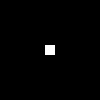
\includegraphics[width=0.25\linewidth]{env_examples/env0.jpg}
    \caption{Example of the simplest environment with a static square.}
    \label{fig:env0}
\end{figure}

I expected the model to overfit quickly since the state was always identical. It reached an average IoU of 0.94 after around 160,000 time steps, but it started to critically forget shortly after, and it never recovered. Nonetheless, the environment was successfully solved. Since this behavior occurred less frequently in the more complex environments, I assume the problem was too simple for a complex algorithm such as \texttt{PPO}.

Figure~\ref{fig:v0_rew} shows the mean reward per episode during the training. Because each episode consists of a single observation, the maximum achievable reward is one, corresponding to a perfect IoU. The $x$-axis shows the elapsed time steps.

\begin{figure}
    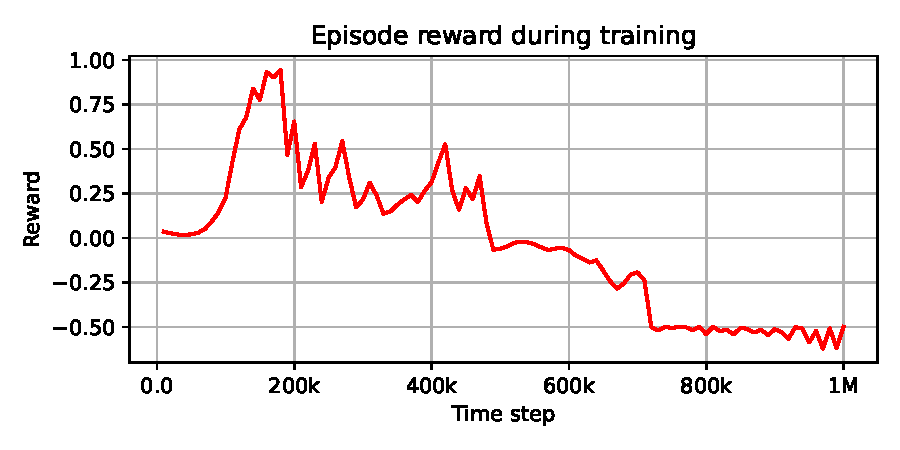
\includegraphics[width=1\linewidth]{graphs/v0.pdf}
    \caption{The mean reward per episode for the simple static square environment. The data was collected by evaluating the agent for 20 episodes after every 10,000 training time steps.}
    \label{fig:v0_rew}
\end{figure}

\section{Randomly placed square environment}
% env v1 %
The next progression involved randomizing the square's position within the image. All the other parameters (reward, action, and algorithm) remained unchanged. Figure~\ref{fig:env1} shows some examples of this environment.

\begin{figure}
    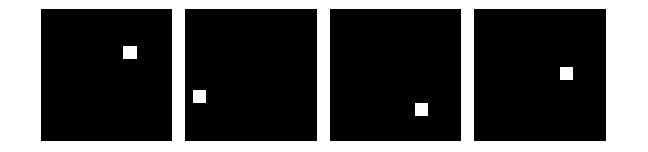
\includegraphics[width=1\linewidth]{env_examples/env1.pdf}
    \caption{Four examples of the environment with a randomly placed square.}
    \label{fig:env1}
\end{figure}

The best-performing model was able to place the bounding box within the region of the square. However, it struggled with accurately predicting the size. In some cases, it predicted a width or height of zero, which consistently resulted in a reward of zero. Similar to the previous model, this one also exhibited catastrophic forgetting. Although the results were suboptimal, the experiment demonstrated that the model could handle varying object positions.

\section{Randomly placed rectangle environment}
\label{sec:moving_rectangle}
% env v2 %
The next environment closely resembled the previous one, with the key difference that the object could now vary in size rather than being a fixed-size square. Both the placement and size were chosen randomly, but with a few constraints. The rectangle’s width and height were constrained to be at least 10 percent of the image dimensions, and its position was restricted to ensure it remained fully within the image boundaries. A few examples are shown in Figure~\ref{fig:env2}.

\begin{figure}
    
\includegraphics[width=1\linewidth]{env_examples/env2.pdf}
    \caption{Four examples of the environment with a randomly placed rectangle.}
    \label{fig:env2}
\end{figure}

In this experiment, I also evaluated the alternative architecture provided by the SB3 library, \texttt{MlpPolicy}. Its architecture has no convolutional layers and no shared feature extractor, more detail is shown in Figure~\ref{fig:mlp_policy} in the Appendix. The network contains fewer parameters (1.3 million versus 2.7 million).

The MLP-based policy outperformed its CNN-based counterpart, and the training progression was more stable. While occasional declines in performance were observed (likely due to exploration), the model consistently recovered and did not exhibit catastrophic forgetting, as shown in Figure~\ref{fig:v2_mlp_cnn}.

\begin{figure}
    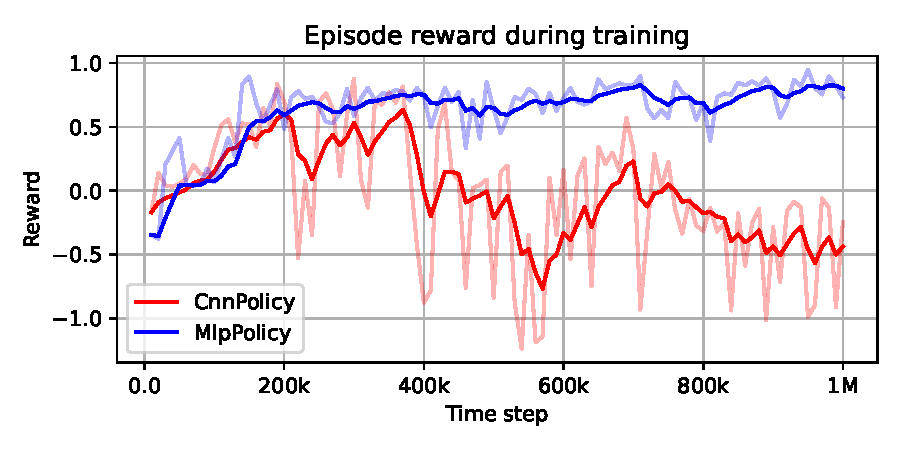
\includegraphics[width=1\linewidth]{graphs/v2_mpl_cnn.pdf}
    \caption{Comparison of the mean reward of the MLP and CNN policies. The data was collected by evaluating the agent for 20 episodes after every 10,000 training time steps. For better clarity, the graph contains both raw values and exponential moving averages.}
    \label{fig:v2_mlp_cnn}
\end{figure}

\section{Multiple rectangles environment}
\label{sec:multi-rect}
% env v3 %
Since the model demonstrated satisfactory performance in detecting a single object, the next logical step was to introduce multiple objects. The next environment had the following properties:
\begin{itemize}
    \item State: consists of a binary $100\times100$ pixel image. Five attempts are made at placing a rectangle of a random size in a random position. It is added to the image if it does not overlap with any already placed rectangles. Because of this randomness, the number of objects changes between episodes, ranging from one to five, with 3.5 being the average. Four examples can be seen in Figure~\ref{fig:env3}.
    \item Action: a tuple of four real numbers representing the bounding box as described in Section~\ref{sec:problem_definition}. If the predicted bounding box overlaps with any objects, those objects are removed from the state entirely, even if the prediction only covers them partially.
    \item Reward: The reward calculation is similar to the previous environments. If the prediction overlaps an object, its IoU with the guess is the reward (if it overlaps multiple, then the maximum IoU is chosen). The episode terminates when all objects are removed. The episode is truncated if the number of guesses matches the number of initially placed objects. It is important to note that the model does not receive a direct penalty for selecting more than one object. However, since only one reward is given, it is more beneficial to select them separately.
\end{itemize}

\begin{figure}
    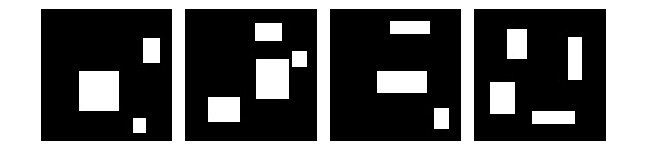
\includegraphics[width=1\linewidth]{env_examples/env3.pdf}
    \caption{Four examples of the environment with multiple randomly placed rectangles}
    \label{fig:env3}
\end{figure}

Both \texttt{MlpPolicy} and \texttt{CnnPolicy} were evaluated. This time, they both performed similarly, stabilizing at a mean reward per episode of around 0.8 after 500,000 time steps. At first glance, the results might seem comparable to the ones in the previous environment. However, since episodes now contained multiple objects, the maximum possible reward per episode increased to, on average, 3.5, in contrast to the previous maximum of 1. This suboptimal result occurred despite both agents executing an average of three actions per episode.

\subsection{Different action definition}
\label{subsec:different_rect_repr}

As mentioned in Section~\ref{sec:problem_definition}, using four real numbers, there are multiple ways to define a bounding box. Before, I interpreted the action as $(x, y, w, h)$. In this experiment, I changed the meaning to $(x_1, y_1, x_2, y_2)$ or the coordinates of the top-left and bottom-right corners. The rationale was that since convolutions are translation-invariant but not scale-invariant, detecting the corners might be easier than detecting the full object, especially when its size varies.

This change slightly improved the performance of the CNN-based model (from 0.8 to 1), but the MLP-based model's performance dropped from 0.8 to 0.5.

\subsection{Transfer from previous environment}

As the previous environment used the same state and action definitions, it was possible to reuse the trained weights in the current environment, enabling the potential for knowledge transfer. Although the transferred agent initially performed better, it quickly degraded and ultimately failed to match the performance of the randomly initialized agent.

\subsection{Changing the network architecture}
\label{subsec:arch_change}

The training trajectories of the experiments in this section exhibited a similar trend. The models initially learned relatively quickly and made significant progress. After the first 200,000 time steps, the progress slowed down dramatically. This plateauing may indicate the agent's network being too simple and unable to learn the optimal strategy.

Since SB3 is built on PyTorch, modifying the underlying neural networks is relatively straightforward. In the default \texttt{CnnPolicy}, the actor and the critic share a feature extractor with three convolutional layers and one fully connected layer. Each of them then includes a single separate fully connected layer (for more detail, see Figure~\ref{fig:cnn_policy} in the Appendix).

Since I had limited experience designing neural network architectures, I consulted ChatGPT for suggestions on a slightly larger design. It suggested adding an extra fully connected layer to the feature extractor and two fully connected layers to the actor and the critic. As a result, the model contained approximately 6 million parameters. The new architecture is shown in more detail in the Appendix in Figure~\ref{fig:bigger_net_policy}.

This new architecture demonstrated a clear improvement. It outperformed the simple network and continued learning even after more than 7 million episodes. Figure~\ref{fig:v3_bigger_net} compares the bigger network and the best \texttt{CnnPolicy} model (the only change between these two experiments was the network architecture).

\begin{figure}
    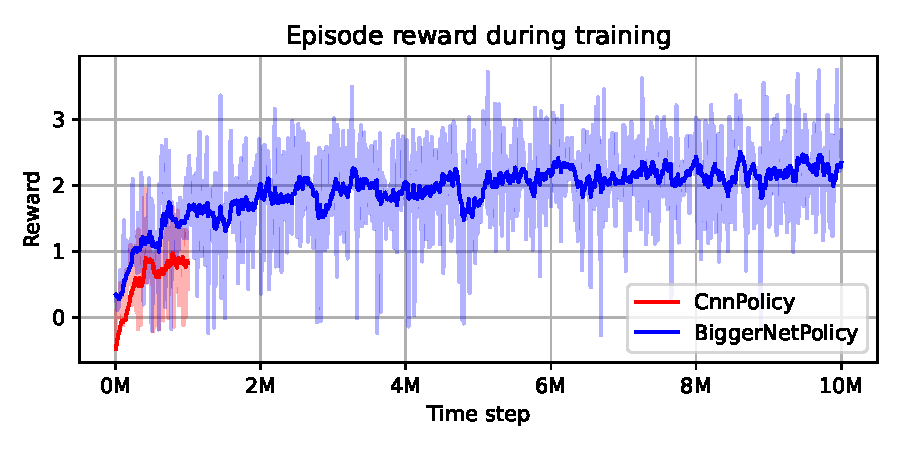
\includegraphics[width=1\linewidth]{graphs/v3_cnn_vs_biggernet.pdf}
    \caption{Comparison of the mean reward of the default \texttt{CnnPolicy} and a bigger network. The data was collected by evaluating the agent for 20 episodes after every 10,000 training time steps. For better clarity, the graph contains both raw values and exponential moving averages.}
    \label{fig:v3_bigger_net}
\end{figure}

The resulting model took around six hours to train and reached a mean reward of around 2.1 per episode or an average IoU of 0.6. One factor that reduced the average reward was that, when the image contained two objects far from one another, the model repeatedly predicted a bounding box positioned between them until the episode was truncated. An example of a situation where this problem occurred can be seen in Figure~\ref{fig:v3_stuck}.

\begin{figure}
    \centering
    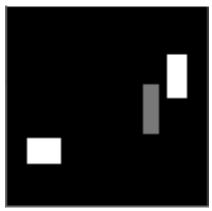
\includegraphics[width=0.25\linewidth]{results/v3_stuck.png}
    \caption{Example of the model getting stuck when two objects are far apart. White rectangles are the actual objects, and gray is the prediction.}
    \label{fig:v3_stuck}
\end{figure}

\section{Environment with objects of different shapes}
\label{sec:different_shapes}
%v4 env%
Now that the model could locate multiple rectangles in a single image, the next step was to introduce other shapes. This new environment was identical to the previous one, but the state could also contain ellipses and triangles instead of just rectangles. Since the rules remained unchanged, there were, on average, 3.5 objects per image, and their bounding boxes did not overlap. Figure~\ref{fig:env4} shows some examples of this environment.

\begin{figure}
    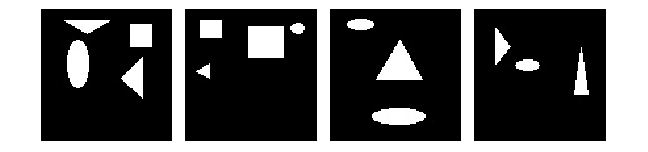
\includegraphics[width=1\linewidth]{env_examples/env4.pdf}
    \caption{Four examples of the environment with multiple different objects}
    \label{fig:env4}
\end{figure}
 
Training with the larger network initially resembled that of the previous environment. However, after 2,500,000 time steps, it stopped learning at a mean episode reward of just over 1.5.

Since the problem was similar to the previous one, I tried using transfer learning with the best model from the previous environment. After just 150,000 time steps, it got to a reward of 1.9 and then slowly climbed to a reward of 2.2 for the rest of the training.

This result demonstrated that achieving strong performance in this environment was feasible. However, I wanted to avoid transfer learning until the very end, because if necessary this early on, it would create a very long and impractical chain of models that depend on one another. Therefore, I aimed to improve the network architecture further.

\subsection{ResNet-18 feature extractor}
\label{subsec:resnet}

It is common practice not to design a feature extractor from scratch but to use one derived from a network pre-trained on a similar task~\cite{DLforVisualSystems}.

ResNet is a model architecture first proposed in the paper \textit{Deep Residual Learning for Image Recognition}~\cite{ResNet18}. It introduced multiple architecture sizes, such as ResNet-18, ResNet-34, ResNet-50, and more.

ResNet-18 is a convolutional neural network with 18 layers and residual (skip) connections that help mitigate vanishing gradients. Each convolution is typically followed by batch normalization. While the original ResNet ends with an average pooling layer, the PyTorch implementation uses an adaptive average pooling layer, which ensures a fixed-size output regardless of the input dimensions.

A minor complication is that ResNet-18 accepts color images with three channels as input, whereas the environment produces binary images with a single channel. To solve this issue, I added a convolutional layer at the beginning with a $1\times1$ kernel, which transforms the single binary channel into three feature maps. The entire architecture is shown in the Appendix in Figure~\ref{fig:resnet_arch}. I also removed the last fully connected layer that is normally used for classification.

It is important to note that the ResNet-18 weights provided by PyTorch were pre-trained on the ImageNet-1k v1 dataset~\cite{torchvision2016}. As this dataset is quite different from my use case, the positive effects of the pre-trained feature extractor could be lowered.

I tried again in the same environment. At first, I used the weights from PyTorch and froze them because I thought this would speed up the training. The results were unsatisfactory, reaching a mean episode reward of 0.5 after 200,000 time steps and not improving further. Next, I ran the same test, but this time, the weights were no longer frozen and could thus adapt to the new problem. In this test, the training performance improved significantly, achieving a reward of approximately 2.8 in under 2.5 million time steps.
To test whether it was the larger feature extractor or the pre-trained weights that caused this improvement, I ran another experiment, where the feature extractor was initialized randomly. This experiment resulted in a mean episode reward of under 2, proving the importance of pre-trained weights. The comparison of these three experiments and the best result reached with the previous architecture can be seen in Figure~\ref{fig:v4_resnet_graph}. 

\begin{figure}
    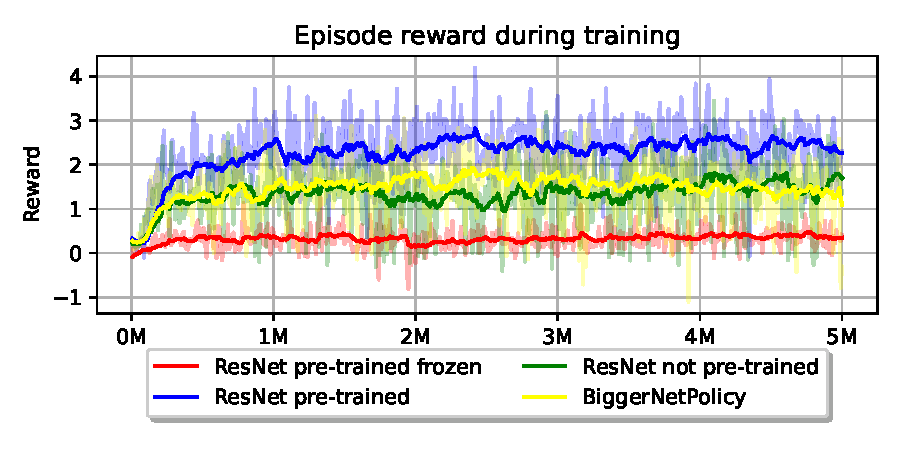
\includegraphics[width=1\linewidth]{graphs/v4_resnet_graph.pdf}
    \caption{Comparison of the mean reward of the pre-trained frozen, pre-trained fine-tunable, and not pre-trained ResNet-18 based agents with the previous architecture. The data was collected by evaluating the agent for 20 episodes after every 10,000 training time steps. For better clarity, the graph contains both raw values and exponential moving averages.}
    \label{fig:v4_resnet_graph}
\end{figure}

Although the performance improvement was substantial, it significantly increased the training time. Training one million time steps required approximately 2.5 hours, which was about three times longer than with the previous architecture.

\section{Environment with hollow shapes}
%env 5%
A significant simplification in the current setup is that each pixel in the image can belong to at most one object. To allow one object to appear inside another, only its outline must be drawn. Otherwise, the inner object would be obscured. The next environment implemented this change. Objects were drawn as outlines, as illustrated in Figure~\ref{fig:env5}. This modification had minimal impact on the training performance.

\begin{figure}
    \centering
    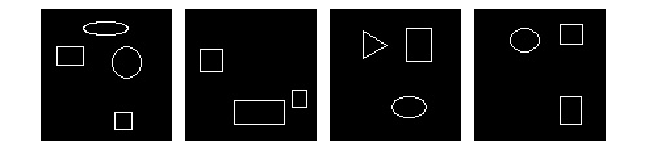
\includegraphics[width=1\linewidth]{env_examples/env5.pdf}
    \caption{Four examples of the environment with multiple shapes of objects where only outlines are drawn.}
    \label{fig:env5}
\end{figure}

\section{Bigger images}
%env 6%
At this point, I was working with images of size $100\times100$ pixels, whereas AIVA currently uses a resolution of $1920\times1080$ pixels. Since object localization does not require pixel-level precision, some downscaling is feasible. However, reducing the image to $100\times100$ pixels is likely too aggressive. To address this problem, I experimented with larger image states.

The largest image resolution at which training could be initiated was $640\times480$ pixels, since with bigger resolutions, the GPU memory size was not sufficient. However, even then, the training speed slowdown was so significant that I continued with a state size of $200\times200$ pixels, which still slowed down the training by a factor of two.

The size increase did not cause significant differences in the training progression. However, since the image was bigger than before, more objects were placed (seven on average). The model learned to place large bounding box predictions in relevant areas. This strategy resulted in a positive reward but was far from optimal. This behavior was likely due to the reward function not explicitly penalizing the selection of multiple objects in a single prediction. To address this, I proposed two alternative algorithms for computing the reward when the predicted bounding box intersects multiple objects:

\begin{itemize}
    \item Find all objects that intersect with the guess. Find the object with the biggest overlap and calculate its IoU. Calculate the sum of the overlap areas of all the other intersecting objects with the guess, divide this sum by the area of the predicted bounding box, and subtract it from the IoU.
    \item Calculate IoUs of all the objects that intersect with the guess. The reward is the biggest IoU minus the sum of all the other IoUs multiplied by a constant.
\end{itemize}

The first option did help, bringing the per-object IoU from 0.5 to around 0.6. The second one had a very minimal impact. Although an IoU of 0.6 is generally regarded as acceptable~\cite{DLforVisualSystems}, this experiment indicated that the current solution struggled even with fewer than ten objects, which is concerning given that a typical website contains many more.

\section{Hierarchical environment}
\label{sec:hierarchical-env}

Up to this point, all environments contained non-overlapping objects. They were independent, meaning the order in which they were selected had no impact. This differs from how actual websites look. They have a hierarchy of objects (one can contain many others). The next step was to create an environment that would represent this structure more faithfully.

Initially, I attempted to use the same technique of randomly placing non-overlapping objects. However, this time I permitted overlaps where one object was entirely contained within another. This strategy was ineffective. The number of objects varied widely between attempts, objects were placed too closely together, and the resulting hierarchies were shallow. So, instead, I created a generator that directly created a tree-like structure.

The generator begins with a root object that spans the entire image. It then selects an internal region with a random offset relative to the parent object and randomly selects the number of children, their sizes, and the spacing between them. The algorithm then does this recursively for each child. The maximum depth, the minimum size of an object, the minimum spacing, and the number of children are customizable. Examples of this hierarchical structure are shown in Figure~\ref{fig:env7}.

\begin{figure}
    \centering
    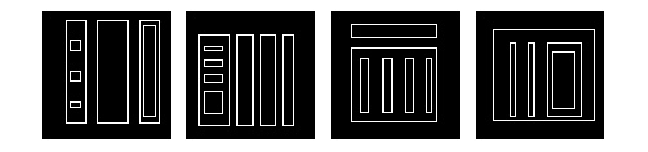
\includegraphics[width=1\linewidth]{env_examples/env7.pdf}
    \caption{Four examples of the new hierarchical environment}
    \label{fig:env7}
\end{figure}

A new reward function was needed as well. I devised and implemented the following method. First, identify all objects that the predicted bounding box either intersects or fully contains. If none are found, include any object that fully contains the prediction (at minimum, this will always be the root object). If only one such object exists, the reward is calculated as the IoU between the predicted box and the object, minus the percentage of the object’s area that is occupied by unguessed child objects. The selected object, along with all its descendants, is then removed from the environment. If multiple intersecting objects exist, the one deepest in the hierarchy is chosen, and the same calculation is performed. The episode terminates when the root object is removed.

I tested this new environment by training two new models. One with randomly initialized weights and the other transferred from the best model in the previous environment. After 7 million time steps, both models achieved an average reward of around 2. A model transferred from the previous environment performed better, but not by much, reaching at most 2.4. From the testing, it was clear that the model learned that placing long bounding boxes of zero width would almost always result in a nonnegative reward. The model failed to explore sufficiently and did not discover more optimal strategies.

\subsection{Manual hyperparameter tuning}

Until this point, I had not experimented with hyperparameters. Since I needed to encourage exploration, this seemed like a good opportunity. I manually experimented with the following parameters:

\begin{itemize}
    \item The discount factor $\gamma$ (described in Section~\ref{sec:goal}) -- By default, this parameter is set to 0.99. Given the environment’s design, each episode has a fixed maximum number of steps, and an optimal policy is expected to utilize all available steps. Thus, discounting is unnecessary, and $\gamma$ should be set to 1.
    \item Entropy loss coefficient $c_2$ -- The PPO loss function contains an entropy bonus that rewards less deterministic policies. Increasing it should thus lead to a more stochastic model and more exploration~\cite{PPO_paper}. By default, this hyperparameter is set to 0.
    \item Clipping range $\epsilon$ -- One of the main benefits of PPO is its clipping function that prevents large updates to the policy and value function, which should prevent it from making drastic changes~\cite{PPO_paper}. By increasing it, the training might become more unstable, but it also might help to get out of local maxima.
    \item Learning rate $\varepsilon$ -- When updating the policy network, the gradient is multiplied by the learning rate. A higher learning rate should make the training faster, but at the same time, the jumps are more significant, which can lead to unstable learning.
\end{itemize}

I experimented with both increasing and decreasing each of these parameters; however, none produced a substantial improvement in performance. Later, when I discovered Optuna (see Section~\ref{sec:optuna}), I also attempted an automated hyperparameter search, but even that had minimal impact. With few remaining options for improving training performance, I opted to explore an entirely different approach.

\section{Switching to discrete actions}
\label{sec:iterative}

Since the results of the previous approach, where bounding boxes were predicted directly, with one action corresponding to one complete prediction, were unsatisfactory, particularly in more complex environments, I decided to try a different method. In~\cite{rl_object_detection}, Samiei and Li describe and compare two previously proposed approaches for object detection using reinforcement learning, both using a discrete action space. Both of these methods start with a bounding box spanning the entire image. Then, the agent chooses actions that modify this selection repeatedly. Once the model is satisfied with the prediction, it selects the \enquote{trigger} action, which confirms the selection. The initial observation includes the entire image (scaled to some fixed size). After each action, the observation is modified to only include the current selection.

The first method, initially described in~\cite{hierarchical_od_with_drl}, has five movement actions (each resulting in zooming towards one of the corners or the center of the image) and the trigger action. It showed promising results for single-object, single-class detection. However, it is unsuitable for this work because it only produces bounding boxes with the same aspect ratio as the image.

The second method, initially described in~\cite{iterative_od_with_rl}, uses a similar approach. However, instead of five actions for zooming in different areas, it has a total of eight movement actions (plus the trigger), four of which move the bounding box (up, down, left, and right), two change the size (zoom in, zoom out) and two change the aspect-ratio (making the selection fatter or taller). These actions allow for way more flexibility, although some bounding boxes remain unreachable due to the discrete nature of the actions. However, if the step size is sufficiently small, this is acceptable, as pixel-perfect predictions are not required. Figure~\ref{fig:exmaple_from_paper} shows an example of one episode using this approach from the original paper.

\begin{figure}
    \centering
    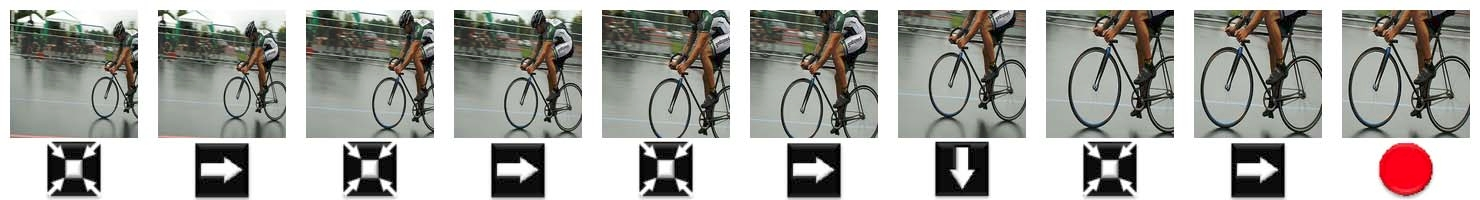
\includegraphics[width=1\linewidth]{diagrams/45.jpg}
    \caption{Example of one episode using the strategy described in~\cite{iterative_od_with_rl} (also the source of the image). The image shows the individual observations and actions taken.}
    \label{fig:exmaple_from_paper}
\end{figure}

As previously described, the observation space is an image. The original paper~\cite{iterative_od_with_rl} also used a vector of ten previous one-hot encoded actions, but Samiei and Li found that excluding this vector did not change the outcome~\cite{rl_object_detection}.

I implemented a simplified version of this approach using only four actions, each reducing the bounding box by a fixed percentage from one of its four sides. This simplification reduces complexity while preserving the ability to produce bounding boxes of arbitrary size.

The proposed reward function compares the IoU before and after an action. A reward of $+1$ is given if the action improves the IoU, and $-1$ otherwise. When the trigger action is selected, a reward of $\eta$ is given if the resulting IoU is over some threshold $\tau$, $-\eta$ otherwise. The suggested values are $\eta=3$, $\tau=0.5$.

This reward function is suitable for single-object detection. However, when more than one object is present, it is difficult to determine whether the action improved the selection since it can differ for each object. For this reason, I started my experiment with a simpler semi-sparse reward function, which only rewards the trigger actions. The same calculation was used as in the corresponding continuous-action environments.

\section{Randomly placed rectangle environment with discrete actions}

To test this new approach, I modified the environment described in Section~\ref{sec:moving_rectangle}, which contains only a single rectangle. The model learned to locate the rectangle, but the accuracy was suboptimal (IoU of 0.4), primarily because the selection reduction was too large (one step reduced the bounding box by 15 percent). The accuracy improved (IoU of 0.7) when the step size was reduced to 5 percent. However, it took on average 60 time steps to locate the object, which slowed down the inference.

Compared to the previous approach in the same environment, training required approximately ten times as many time steps to reach the same reward. This increase was expected, as a single prediction now required 30 to 50 time steps instead of just one.

\section{Multiple rectangles environment with discrete actions}

Since the results in the simple single-rectangle environment were satisfactory, I continued and modified the environment described in Section~\ref{sec:multi-rect} to use discrete actions. To address the accuracy issues caused by large step sizes in the previous environment, I implemented two actions per direction: one that reduced the bounding box by 15 percent and another that reduced it by 2.5 percent. Although this change slightly increased the task complexity, it enabled more precise predictions using fewer steps.

This is the environment in which, under the previous approach, I had to switch to a larger network architecture. This time, I started directly with the ResNet-18-based network. This configuration performed well, achieving a mean episode reward of 2.1 in approximately 700,000 time steps, significantly fewer than the 10,000,000 required by the previous approach, even though each episode took around 80 time steps compared to just 3.5 previously.

\section{Hierarchical environment with discrete actions}

Given the success of the new approach, I proceeded to test it on the hierarchical environment described in Section~\ref{sec:hierarchical-env}, which I had previously been unable to solve using continuous actions.

\subsection{Changing to dense reward function}

Unfortunately, this new approach did not lead to improved performance. The agent struggled even to reach positive rewards. I decided to modify the reward function to more closely align with the one described in~\cite{iterative_od_with_rl}. The primary modification involved changing from a semi-sparse reward function, which only provided feedback for trigger actions, to a dense reward function that assigned rewards for every action.

I devised the following reward function. After each interaction, find all leaf objects (with no children) that overlap with the current selection. If no such elements are found, a reward of zero is given. Otherwise, find the element that has the highest IoU with the current selection. If the selected action is the trigger action and the IoU exceeds 0.5, a reward of 3 is given; otherwise, a reward of -3 is assigned. In both cases, the element is removed from the observation. If it is not the trigger action, compare the IoU with the previous best IoU and reward the difference. The episode ends once all nodes are removed.

After further experimentation, I modified the trigger action reward to scale with the IoU, awarding three times the IoU value. This change was made to encourage the agent to surpass the threshold IoU of 0.5, which a fixed reward failed to incentivize.

\subsection{Automated hyperparameter tuning}

Since there was little progress, I decided to revisit hyperparameter tuning, but this time using Optuna (see Section~\ref{sec:optuna}).

I ran a study of 200 trials, each running 200,000 time steps (unless terminated earlier due to pruning). The entire tuning process spanned approximately 24 hours. However, the optimal hyperparameters were identified in trial 23 within the first 3 hours. According to this study, the most important hyperparameter was the learning rate. Reducing the default learning rate to approximately one-tenth, combined with linear decay, yielded a notable improvement in performance.

The new reward function and hyperparameters brought the average episode reward from barely over 0 to over 12 in less than 1,000,000 training time steps. Given that the environment generated an average of 3.9 objects per episode, and the maximum attainable reward per object was 4 (1 from shrinking actions and 3 from the trigger action), this outcome corresponds to an average IoU exceeding 0.75.

After increasing the average amount of objects per image to 6.3 and another two days of hyperparameter tuning, the reward reached 20, or an IoU of almost 0.8 per object. These results demonstrated that the discrete-action approach scaled effectively with increasing object counts.

One of the tunable parameters was the size of the actor and critic networks. In both tuning sessions, this parameter was found to have minimal impact on performance. In that second one, the best result was achieved using the smallest architecture, where, apart from the shared feature extractor, both the actor and the critic consisted of only one layer of 64 neurons. This result prompted me to revert to the simple \texttt{CnnPolicy} provided by SB3.

\section{Environment with objects based on website screenshots}
%v8 env%

Having successfully trained a model to detect elements in a hierarchical environment, I proceeded to experiment with more realistic data. Rather than placing rectangles at random, I aimed to base their position and size on the structure of real websites.

\subsection{Dataset}
\label{subsec:dataset}

Ideally, I aimed to find a dataset containing website screenshots with corresponding element annotations. Such datasets do exist, for example, those presented in~\cite{roboflow-dataset-1, roboflow-dataset-2}. Unfortunately, they are small (at most a bit over 1,000 images), contain only the leaf elements (i.e., the smallest visual components), and exclude larger structural sections such as spans or divs, and often contain straight-up wrong or duplicate annotations. This limitation reinforces the motivation for this thesis, which aims to train a DL-based model without relying on such annotated datasets.

Instead, I chose to use a dataset that contains just the screenshots and then estimate the approximate locations of elements using a CV-based function. The best public dataset I found was~\cite{aydos2020}. This dataset contains 20,000 website screenshots split into four categories: machinery, music, sport, and tourism (the original purpose of the dataset is to classify these categories). It provides screenshots in two resolutions: $224\times224$ pixels (which are too small for this application) and $1440\times900$ pixels.

For each image, I identified the elements using the following method. First, convert the image to grayscale and apply a bilateral filter, which reduces the impact of textured backgrounds that could interfere with edge detection. Next, locate edges using the Canny edge detection algorithm, and connect close ones using morphological closing. Finally, connected components are identified, and those below a minimum size threshold are discarded. A new black image of the same dimensions as the original screenshot is created, and white rectangles corresponding to the detected objects are overlaid. The result is similar to what I generated in the last environment, but based on an actual website. Since the original image is not provided to the model, occasional missed detections do not pose a significant issue. The individual steps are shown in Figure~\ref{fig:simple-detector}.

\begin{figure}
    \centering
    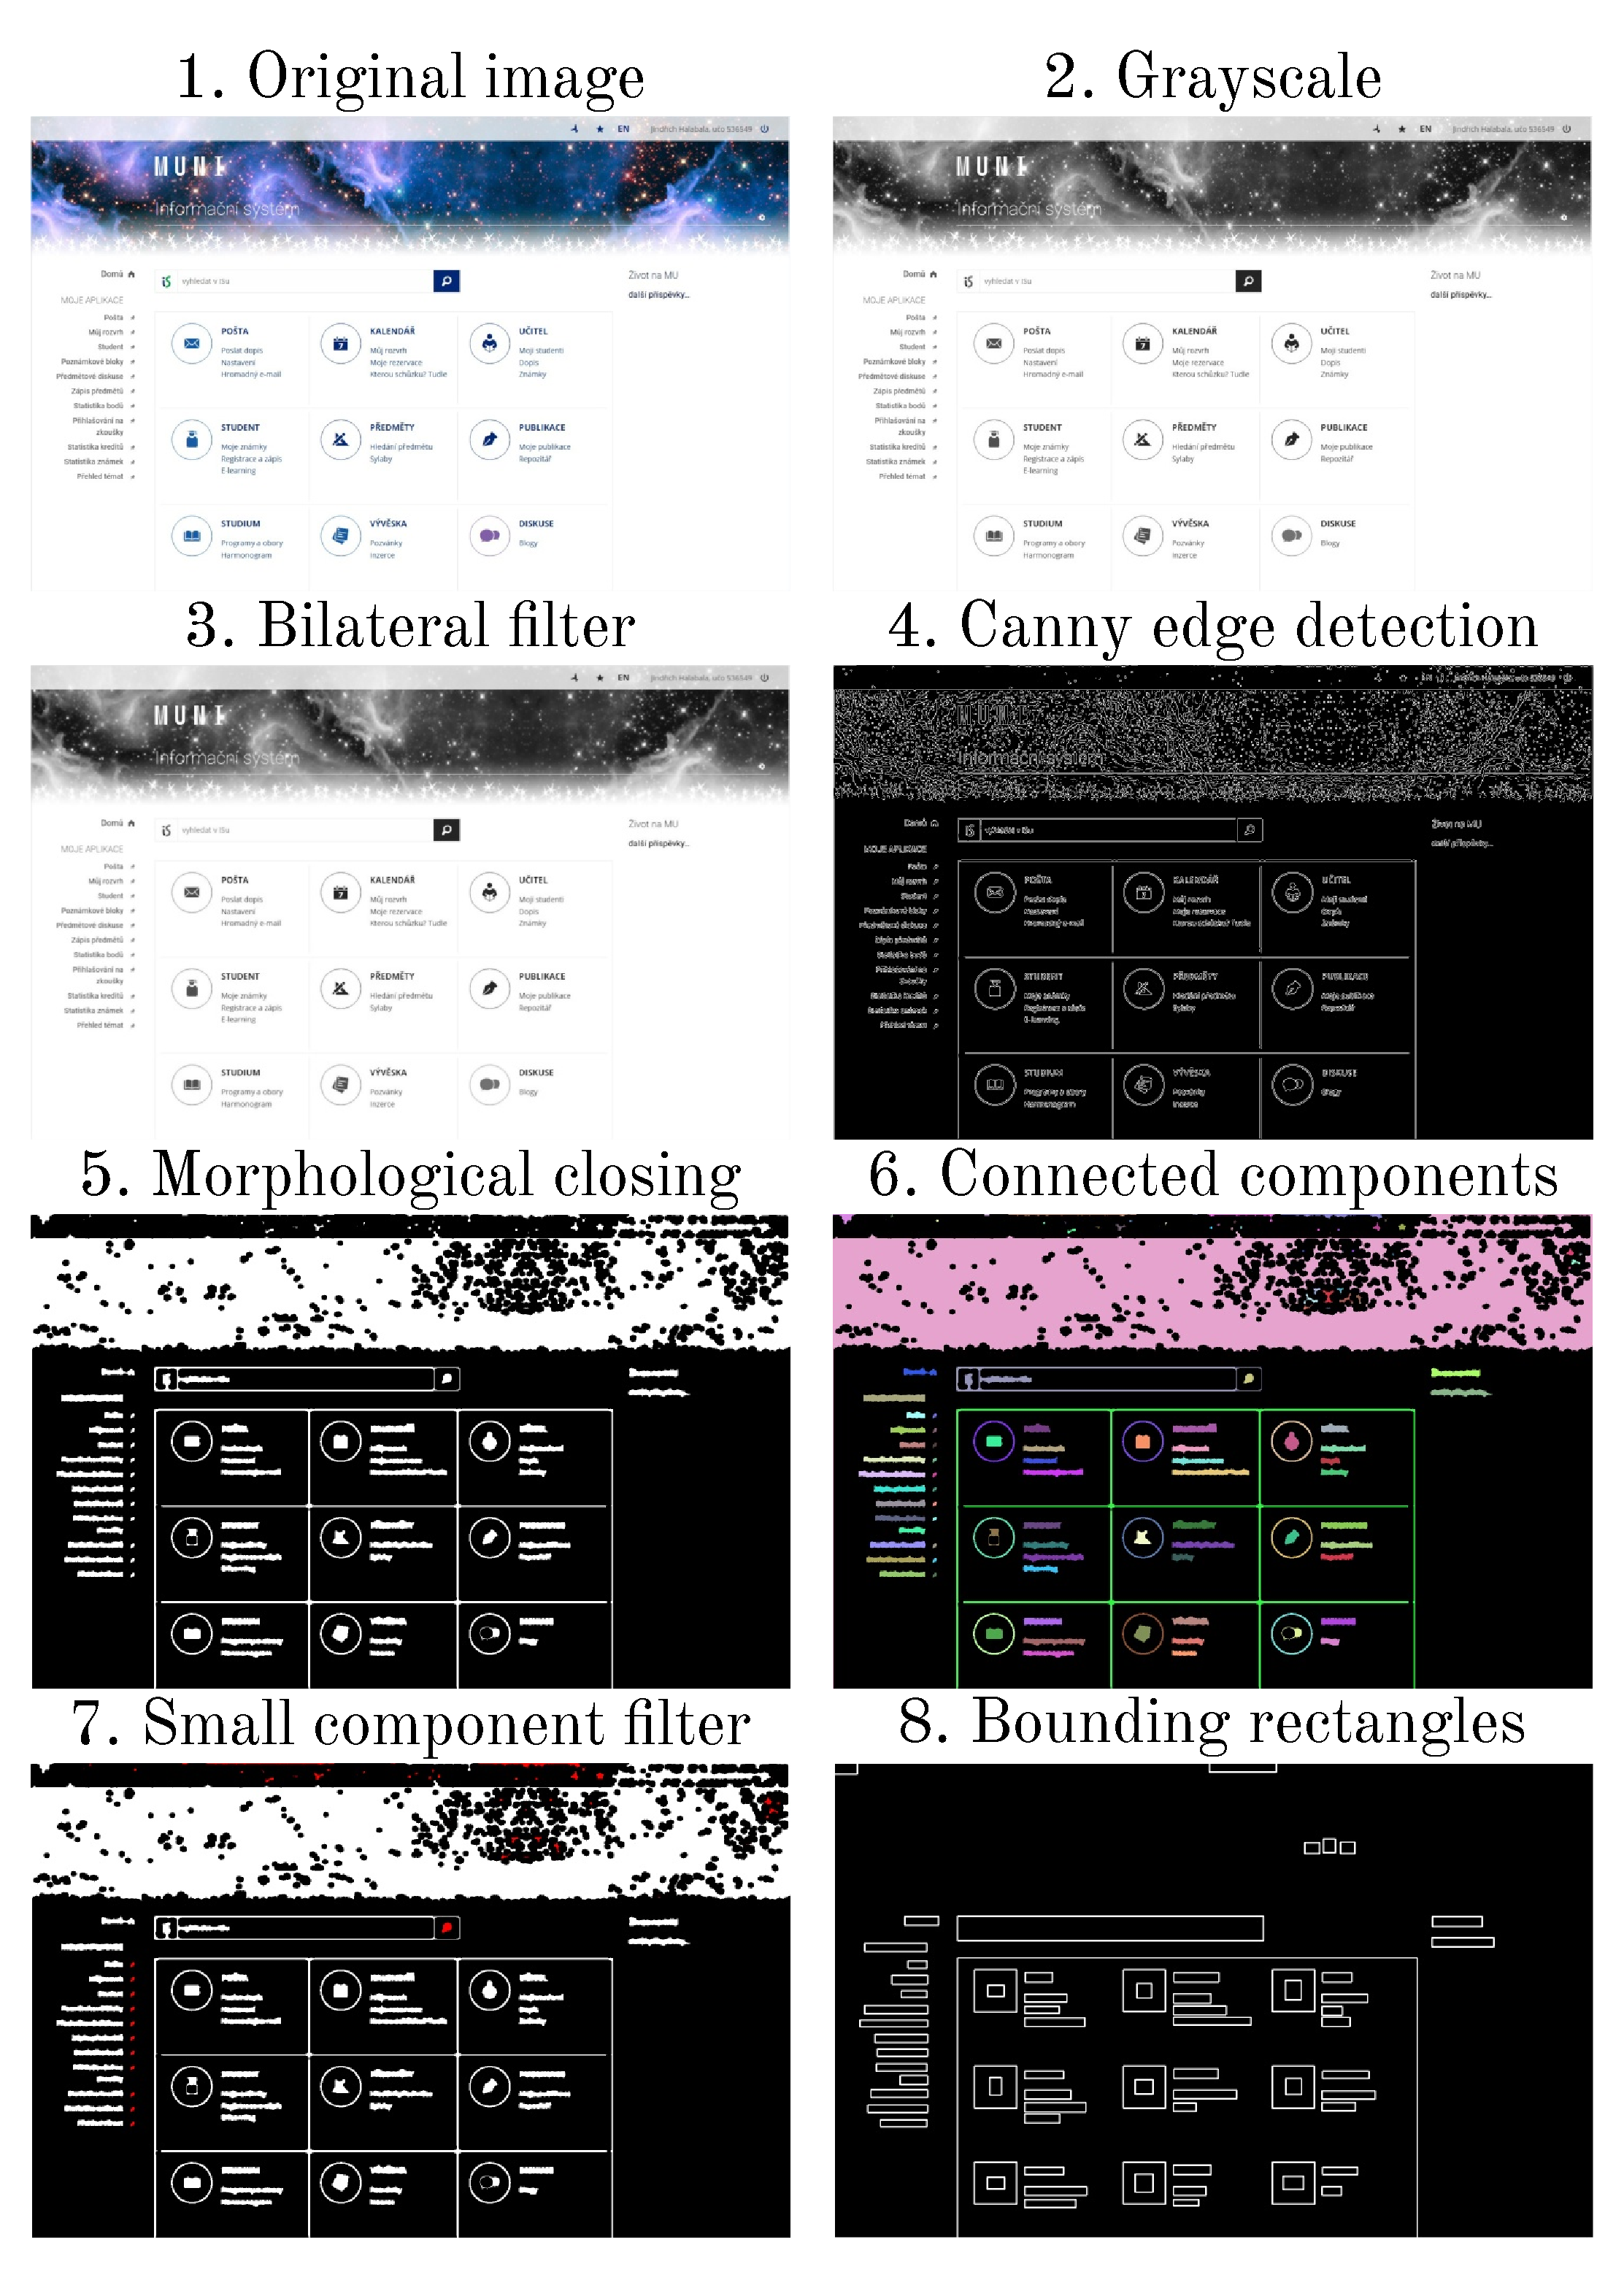
\includegraphics[width=1\linewidth]{diagrams/simple_detector.pdf}
    \caption{The steps taken when creating a state from an image.}
    \label{fig:simple-detector}
\end{figure}

Using this method, an average of 26 objects per image was detected. Assuming a target IoU of 0.7 under the current reward function, the goal episode reward for this environment was approximately 72 per episode. A few examples of the initial states are shown in Figure~\ref{fig:env8}.

\begin{figure}
    \centering
    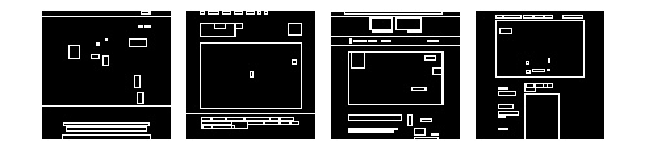
\includegraphics[width=1\linewidth]{env_examples/env8.pdf}
    \caption{Four examples of the environment where rectangles are based on real websites.}
    \label{fig:env8}
\end{figure}

\subsection{Reward function}

At first, I reused the reward function from the previous environment. In that setting, with fewer than 10 objects, the function performed reasonably well. However, when the number of objects exceeded 20, the agent failed to learn effective behavior. The resulting model repeatedly placed large predictions until the episode terminated.

To address this issue, I modified the logic to consider not only leaf objects. If the initial prediction was large and achieved the highest IoU with the root element, the episode was terminated immediately. Unfortunately, this brought yet another problem. Since the initial selection is identical to the root element, the next couple of actions would always result in negative rewards. The selection would worsen until it became small enough to have a better IoU with another element. To mitigate potential confusion caused by consistently negative rewards, I added a condition that excluded the root element from calculations unless it was the only remaining object.

Following this modification, the model achieved an average reward of approximately 20 per episode.

\subsection{Curriculum learning}

Curriculum learning is a technique where the agent is trained on data of increasing difficulty. Since the states were still generated manually, implementing this strategy was relatively straightforward. Initially, only the $n$ largest bounding boxes were included during image generation. At the start, I set $n=3$. I stored the rewards in an array, and once 100 values were collected, I computed their average. If the average exceeded a predefined threshold (initially set to 0.7), I incremented $n$ by one.

After 20,000,000 training steps with curriculum learning, the agent outperformed its previous mean reward per episode by 5. More importantly, the reward continued to increase even after prolonged training, indicating sustained learning progress.

Subsequently, I identified additional issues in the environment. Specifically, the reward for non-trigger actions, calculated as the difference between the current best IoU and the previous best IoU, was ineffective when applied immediately after a trigger action.
Another notable issue concerned image scaling. Since the RL algorithms require the same-sized input every time, it was necessary to scale the selection to the state size. The problem is that, based on the interpolation method used when scaling, some lines could be lost during interpolation, rendering them undetectable to the agent. Especially problematic was that this scaling could be both up-scaling and down-scaling, or even both, one for each axis. This issue was resolved by applying independent scaling for each axis and selecting the interpolation method adaptively based on the situation.

After addressing these issues, the agent achieved an average reward of 55 per episode.

\subsection{Tolerant Intersection over Union}
\label{subsec:eval_metric}

Up to this point, I used the Intersection over Union (IoU) metric to evaluate the quality of a bounding box selection. IoU is the standard metric for evaluating predicted bounding boxes against ground truth annotations. It performs effectively in conventional object detection tasks where objects are generally of similar size. However, this assumption does not hold in the current setting. Some objects can take up most of the image, while others can take up less than 0.01 percent of the screen area.

Because IoU reflects relative error, it does not align well with the objectives of this work. The task prioritizes absolute differences in bounding box positions and sizes over relative errors. For instance, a 2-pixel deviation on a small element is acceptable, despite its high relative error. Conversely, a 50-pixel error on a large element is problematic, even if it constitutes a small relative discrepancy. For this reason, I wanted to experiment with other metrics that could better reflect my requirements.

Since the agent receives only a zoomed-in view of the image, introducing a metric that depends on the selection’s size would violate the Markov property. The model cannot distinguish whether it is highly zoomed in on a small object or minimally zoomed in on a large one. To address this limitation, the observation space was expanded to include the coordinates of the current view window. This required transitioning to the \texttt{Dict} observation space and implementing a new feature extractor that concatenates these coordinates to the features extracted from the image. The complete architecture of the modified network is illustrated in Figure~\ref{fig:multiinput_arch} in the Appendix.

This modification alone led to a substantial acceleration in training, achieving a stable mean episode reward of 60 in less than one-third the number of time steps and eventually reaching a mean episode reward of over 70, even though it should not be needed with regular IoU.

The first alternative metric I created is Tolerant Intersection over Union (TIoU). This metric introduces an additional tolerance parameter. Prior to computing the IoU, the edges of the two bounding boxes are moved closer together by up to the specified tolerance value (defined in absolute terms). The final score is computed as a weighted sum of the IoU of the original and adjusted bounding boxes, maintaining a preference for precise matches.

This new metric mitigated the sensitivity of small bounding boxes to minor errors, resulting in a reduction of average episode length by nearly 100 steps, to approximately 750. However, it did not improve inaccurate selections involving large bounding boxes, because the metric can never produce a worse score than regular IoU.

\subsection{Absolute Sigmoid Score metric}

Since the Tolerant IoU metric did not solve the issues with large bounding boxes, I aimed to construct a metric based solely on absolute differences, independent of box size.

The Absolute Sigmoid Score metric computes the differences between the minimum $x$ and $y$ coordinates of the two boxes, the maximum $x$ and $y$ coordinates, and the $x$ and $y$ coordinates of their centers. The sum of these differences (marked as $\text{Diff}( b_1, b_2)$ in the formula below) is then passed through a sigmoid function with a descending shape, achieved by subtracting it from one. The sigmoid constrains the result to the $[0,1]$ interval and reflects the intuition that smaller differences should be penalized less. The sigmoid function has two parameters, $\alpha$, which controls the steepness of the sigmoid, and $\theta$, which shifts the sigmoid (I used values $\alpha = 2.8$ and $\theta = 0.5$). To ensure that a perfect match always yields a score of one, regardless of $\alpha$ and $\theta$, the result is divided by the value of the sigmoid at a difference of zero.

\begin{equation}
\begin{split}
    \sigma(x) & = \frac{1}{1+e^{-x}} \\
    \text{AbsSigScore}( b_1, b_2) & = \frac{1-\sigma(\alpha\cdot(\text{Diff}( b_1, b_2)-\theta))}{1-\sigma(-\alpha\cdot\theta)}
\end{split}
\end{equation}

I struggled to find a suitable threshold at which the score could be considered good enough to increase the difficulty of the curriculum learning. 0.85 was too low, resulting in a model with inaccurate predictions; 0.9 was too high for the model to reach, and the training did not progress. It is possible that with different values of $\alpha$ and $\theta$, this metric might be suitable. Nevertheless, for the rest of the experiments, I returned to TIoU.

\subsection{Selection padding}

One potential issue I noticed when debugging the environment was that the agent observes only the current selection. Since the objects are only represented by their outline, the agent can no longer see one of the object's edges if it overshoots while shrinking the selection. Given that the agent has no memory, this limitation could pose a challenge. I addressed this by enlarging the observation window by a fixed percentage on each side to include some extra area around the selection.

Although the final performance after 20 million training steps was nearly identical (stable mean episode reward of around 80 per episode), it did learn faster, especially at the beginning.

\section{Finding objects in a real image}
%v9 env%

The previous environment showed that it is possible to train a model capable of finding objects even in relatively complex hierarchies. However, it was still locating only rectangles in a heavily preprocessed image. This preprocessing required detecting all objects in advance using a separate method, thereby diminishing the practical value of the model. The next step was to create an environment with only minimal image preprocessing that does not require prior knowledge of object locations. The environment processes a website screenshot by detecting edges and expanding them using morphological dilation. Figure~\ref{fig:env9} shows some examples of the state the model receives.

Apart from the change in the observation space, this environment was similar to the previous one. The reward was still calculated based on ground truth labels. However, this time I used a more advanced CV-based detector (described in Section~\ref{sec:trad_cv_detector}) to increase the reward function's accuracy. This increased the average number of detected objects per image to 32.4, implying an optimal mean episode reward of 129.6. The target reward was set at 90 per episode (corresponding to a TIoU of 0.7).

\begin{figure}
    \centering
    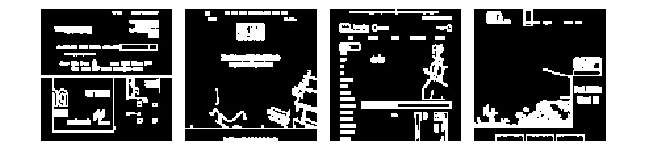
\includegraphics[width=1\linewidth]{env_examples/env9.pdf}
    \caption{Four examples of the environment where the state is a slightly preprocessed image.}
    \label{fig:env9}
\end{figure}

When training in this environment using the same setup as before, the agent achieved a peak mean episode reward of 46.

The first modification involved changing the method used to scale the image. In the previous environments, the image was always binary. This was because the objects were marked by only a one-pixel-wide outline, which would nearly disappear when the image was significantly downscaled. Here, this was no longer the case. By preserving all 256 grayscale pixel values, the model gained access to richer visual information, enabling it to discern finer details. As a result of this change, the average episode reward increased from 46 to 53.

\subsection{Changing the feature extractor}
\label{subsec:feat_extract_two}

As discussed in Section~\ref{sec:different_shapes}, adapting to variations in object shapes necessitated a larger feature extractor. As a reminder, after switching to a discrete action space, the later environments were solved using a network with a simple, non-pretrained feature extractor consisting of only three convolutional layers. Since the reward decreased significantly with the introduction of more complex objects, a larger feature extractor could offer improvements.

When using the larger network developed in Subsection~\ref{subsec:arch_change}, modified to incorporate the selection's coordinates, the mean episode reward increased from 53 to 62. In contrast, when using the ResNet-based architecture (Subsection~\ref{subsec:resnet}), the model's performance rapidly deteriorated to a mean reward of zero and failed to recover during training. Based on a suggestion from ChatGPT, I experimented with an alternative pretrained feature extractor, SqueezeNet1.1. Compared to ResNet-18, it contains approximately one-tenth as many parameters while maintaining comparable performance~\cite{torchvision2016}. The new architecture is shown in Figure~\ref{fig:squeezenet_arch} in the Appendix.

Training with the SqueezeNet feature extractor yielded a mean episode reward of approximately 65 after 20,000,000 time steps. Since the mean episode reward was still increasing, I extended the training for an additional 20,000,000 time steps with the learning rate reduced by half. This resulted in a peak mean episode reward of 94 on the validation data. I believe that further hyperparameter tuning and extended training could yield even better results. However, since this single training run took over 33 hours, additional experimentation would be very time-consuming on my current hardware.

\section{Further possible optimizations}
\label{sec:further_optim}

This section outlines additional optimizations that could improve the performance and usability of the RL-based agents.

The current action design results in a slow detector, as each prediction typically requires dozens of individual actions. Adjusting the shrinkage percentage or introducing additional action types could significantly reduce the number of required steps. With the originally attempted continuous actions, a single step per object would be sufficient. A hybrid approach combining discrete and continuous actions, where the model selects both a direction and a shrinkage percentage, could also be effective. However, the SB3 library currently does not support mixed action spaces.

Although the final environment does not rely on ground-truth labels to construct observations, it still depends on them for reward calculation. These labels do not need to be manually provided, as they are generated using a CV-based function. For real-world applications, a reward function that does not require ground-truth labels would be more practical.

This thesis employed only the PPO algorithm for agent training, as it was deemed the most appropriate in Section~\ref{sec:algo_choice}. However, other algorithms may offer improved performance.

Finally, in tasks where ground-truth labels are available, reinforcement learning can serve an alternative role. The model is initially trained using supervised learning for efficiency, and then fine-tuned with reinforcement learning, either using a traditional reward function or by incorporating human feedback. For a system like AIVA, this approach could be particularly practical, as users could provide feedback following a test run. This technique is already widely adopted for the fine-tuning of large language models~\cite{LLM-RLHF}.

\chapter{Comparison with other methods}
\label{ch:comparisons}

In the previous chapter, I described the development of a GUI element detector trained using deep reinforcement learning. While this demonstrated the feasibility of the RL-based approach, it did not assess whether it provides any advantages over traditional methods. In this chapter, I present two prototype detectors based on conventional techniques and compare them to the RL-based approach across multiple criteria.

\section{Traditional CV-based detector}
\label{sec:trad_cv_detector}

To create a detector based purely on traditional computer vision algorithms without the use of machine learning, I combined techniques described in Section~\ref{sec:traditionalCV} to improve the earlier detector described in Subsection~\ref{subsec:dataset}. The primary differences were the use of contour tracing and stricter object filtering. The entire algorithm is described in detail in Appendix~\ref{ap:cv}.

\section{Supervised DL-based detector}

A second common approach to object detection, particularly for more complex images, involves deep convolutional neural networks capable of predicting a variable number of bounding boxes trained using supervised learning.

I chose not to implement such a model from scratch. Instead, I opted for YOLOv8~\cite{yolov8_ultralytics}. It was developed by Ultralytics\footnote{\url{https://www.ultralytics.com/}} in 2023. YOLOv8 is a collection of pre-trained models for various tasks and of multiple sizes (ranging from 2.7 to 99.1 million parameters)~\cite{ultralytics-docs}. Specifically, I used the smallest object detection model \texttt{YOLOv8n}. Although newer versions have since been released, I selected YOLOv8, since I have worked with it previously, and prior studies have demonstrated its effectiveness in detecting GUI elements~\cite{GUI_YOLO_comparison}.

The model is pretrained on the COCO dataset~\cite{COCO} and must be fine-tuned for the specific purpose. As mentioned previously, datasets for my task are limited, so for this prototype, I decided to create my own dataset. To do so, I used my CV-based detector (see Section~\ref{sec:trad_cv_detector}) and labeled 10,000 images from the WebScreenshots dataset~\cite{aydos2020}. It is important to note that this renders any direct accuracy comparison between these two detectors invalid, since the YOLOv8 model is learning to copy the CV-based detector. However, given that all three detectors are prototypes, this limitation is acceptable for the purposes of this comparison. It can be reasonably assumed that if the model performs well on this mocked dataset, it would also generalize effectively when trained on a real annotated dataset.

Fine-tuning the model is straightforward. Using the Python Ultralytics API, an instance of the \texttt{YOLO} class is initialized with the path to a pretrained model. Next, the \texttt{train} method is called with the path to the dataset. The epoch count, early stopping criteria, initial learning rate, and other hyperparameters can be specified. However, if these parameters are not provided, the library automatically determines suitable defaults. Ultralytics also provides a command-line interface.

\section{Challenges of comparing the detectors}

Before comparing the three detectors, it is important to note that each is at a very different level of maturity. The RL and CV-based detectors were developed by me with differing levels of domain expertise and time investment. The DL-based detector was created by professionals and only fine-tuned by me.

These prototypes are sufficient to compare the underlying approaches and draw attention to their main benefits and problems. However, for practical deployment in systems such as AIVA, more detailed comparisons should be done with specific existing detectors.

\section{Accuracy}

In classical object detection tasks, accuracy is measured by comparing the predictions with some ground truth labels. However, in the case of UI element detection, this is problematic due to the presence of multiple valid interpretations. For example, a paragraph of text can be detected as a single element, as one element for each row, one for each word, or even one for each letter. We may prefer one of these options over the others, but none of them is inherently wrong. For this and other reasons outlined in the previous section, no quantitative metrics are reported in this section.

The traditional CV-based detector struggles primarily with detecting text and images. The text grouping is inconsistent, short words are filtered out, and text on a background of similar color is missed completely. While entire images are detected correctly, high-contrast internal content is misclassified as separate elements. Some of these problems are illustrated in Figure~\ref{fig:cv-mistakes}.

\begin{figure}
    \centering
    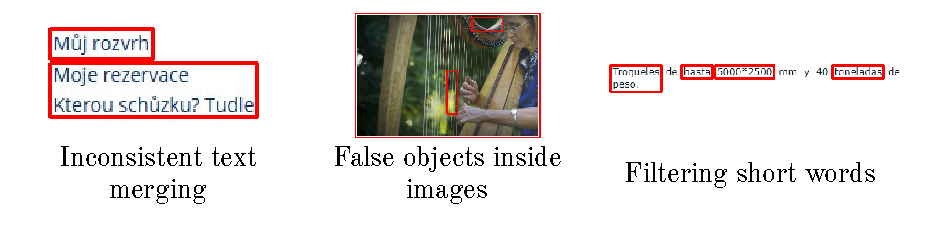
\includegraphics[width=1\linewidth]{diagrams/cv_mistakes.pdf}
    \caption{Examples of common mistakes made by the CV-based detector.}
    \label{fig:cv-mistakes}
\end{figure}

As for the positives, the predictions match the outline of the element well; it does not happen that a prediction is too large or too small. Crucially, when a prediction is incorrect, the cause can be identified and addressed by adjusting the filtering parameters. The white-box nature is, in my opinion, the biggest advantage compared to the other detectors.

Despite being trained on data generated by the CV-based detector, the YOLO-based model ultimately outperformed it. This could be because it was trained only for 100 epochs and thus it did not have time to overfit. Whereas the CV-based detector produced more false negatives (missed elements), this one was more prone to false positives (guessing extra elements). Approximately five percent of the predictions were slightly oversized or undersized on a single edge, which did not happen in the training data. These mistakes are shown in Figure~\ref{fig:yolo-mistakes}.

\begin{figure}
    \centering
    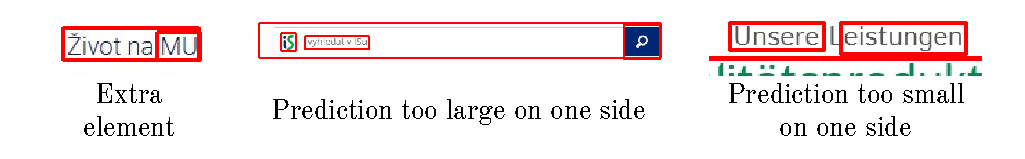
\includegraphics[width=1\linewidth]{diagrams/yolo_mistakes.pdf}
    \caption{Examples of common mistakes made by the YOLO-based detector.}
    \label{fig:yolo-mistakes}
\end{figure}

As the final RL-based detector serves primarily as a proof of concept, its accuracy is not comparable to the other two. Figure~\ref{fig:gov_predict_rl} shows its results on a simple website. While it clearly focuses on the correct areas, the predictions have inaccurate sizes. Since areas of previous guesses are removed from the state, making a large selection can remove other elements and ruin the entire detection, which happened with around 25 percent of images. Overall, the approach shows potential, but a lot more work would have to be invested to make it match the results of the other two methods.

\begin{figure}
    \centering
    
\includegraphics[width=1\linewidth]{results/rl_pred_gov.jpg}
    \caption{Predictions (marked in red) of the final RL-based model on a simple website.}
    \label{fig:gov_predict_rl}
\end{figure}

\section{Speed}
\label{sec:speed}

For real-time applications, the speed of a detector is crucial. AIVA may run tens or even hundreds of detections when testing a website. Thus, the speed of the detector plays an important role.

The prediction times for the YOLO-based detector were by far the fastest. The median prediction time was 12 ms on the GPU and 30 ms on the CPU. The time depended on the number of objects detected, though the differences were small (11 ms for 20 objects, 15 ms for 80 objects). The first prediction was significantly slower, taking approximately 1.5 seconds.

The CV-based detector was slower, with a median prediction time of 144 ms. Here, the object count played a bigger role (125 ms for 20 objects, 200 ms for 80 objects). However, it does not require any initialization, resulting in a shorter time to first prediction than the YOLO-based detector. If speed were the primary goal, it could be further optimized. For example, the bilateral filter takes up over 46 percent of the runtime. Another 17 percent is spent on thousands of operations involving bounding boxes, many of which could potentially be eliminated or computed more efficiently.

The RL-based detector is slower. While each step of the model only takes a bit over 1 ms on the GPU (around 2 ms on the CPU), this approach also requires simulating the environment (around 0.5 ms per step) and, most crucially, every bounding box prediction requires anywhere from 20 to 50 steps. This results in over 100 milliseconds per bounding box and several seconds for a complete image. Some possibilities of improving this are presented in Section~\ref{sec:further_optim}.

%\begin{table}
%    \centering
%    \begin{tabular}{c|cc}
%         & Time to first prediction & Next predictions \\
%         \hline
%         YOLO & 1500 ms &  12 ms \\
%         CV & 144 ms &  144 ms \\
%         RL& 2991 ms &  2048 ms \\
%    \end{tabular}
%    \caption{Caption}
%    \label{tab:my_label}
%\end{table}

\section{Data requirements}
\label{sec:data_req}

Since one of the main motivations for using RL was its potential to be less reliant on large quantities of data, I tested how it compared to the YOLO-based detector on smaller datasets. Both final models were trained on 8,000 images (using half of the 20,000 images from~\cite{aydos2020}, with 1,000 reserved for validation and 1,000 for testing). I repeated the trainings on datasets of 1,000 images and 100 images.

The RL models began training with similar performance. After eight million time steps, they all reached a mean episode reward of approximately 38 on the validation data. After that, their improvement speed started to separate. After 20 million time steps, they were reaching stable episode rewards of 65, 59, and 50, respectively. Performance on the training data showed episode rewards of 25, 25, and 30, respectively. These values are lower due to the curriculum learning strategy, in which more objects are introduced only after the model reaches an average TIoU of 0.7. This clearly indicated that the model trained on the smallest dataset was overfitting to the training data. The model trained on the middle-sized dataset exhibited greater difficulties with generalization than the original, but its episode reward curve ended on an upward trend, suggesting it might continue improving with additional training. The exact values are shown in Table~\ref{tab:rl_results}.

\begin{table}
    \centering
    \begin{tabular}{c|cccc}
        Dataset size & Val. 8M & Train 8M & Val. 20M & Train 20M \\
         \hline
        8,000 & 35.42 & 11.13 & 64.89 & 25.02 \\
        1,000 & 34.97 & 10.72 & 58.73 & 24.96 \\
        100   & 35.91 & 13.91 & 50.36 & 30.15 \\
    \end{tabular}
    \caption{The mean episode rewards of the three agents after 8 million and 20 million time steps on the training and validation data. A higher validation reward is better.}
    \label{tab:rl_results}
\end{table}

The three YOLO models were trained until they stopped improving (no improvement in evaluation metrics for 100 epochs). The values of evaluation metrics on the validation data are shown in Table~\ref{tab:yolo_results}. Visual inspection showed that the model trained on the intermediate dataset performed similarly to the original, except that it often produced duplicate predictions for approximately 10 percent of elements and generated less precise bounding boxes. The model trained on the smallest dataset exhibited similar issues, but these occurred much more frequently, affecting nearly every detected object.

\begin{table}
    \centering
    \begin{tabular}{c|cccc}
        Dataset size & Precision & Recall & mAP50 & mAP50-95 \\
         \hline
        8,000 & 0.738 & 0.715 & 0.770 & 0.626 \\
        1,000 & 0.648 & 0.655 & 0.660 & 0.503 \\
        100   & 0.642 & 0.562 & 0.557 & 0.380 \\
    \end{tabular}
    \caption{The performance metrics of YOLOv8n on different dataset sizes. In all metrics, higher is better.}
    \label{tab:yolo_results}
\end{table}

\chapter*{Conclusion}
\markright{\textsc{Conclusion}}
\addcontentsline{toc}{chapter}{Conclusion}
This thesis experimentally investigated the feasibility of creating a graphical user interface element detector based on deep reinforcement learning. The goal was to explore an alternative to traditional methods that may require less data. The work included the implementation of ten reinforcement learning environments, some with both continuous and discrete action variants. Over 1,000 hours and approximately one billion time steps were spent training agents in these environments using various network architectures, reward functions, and other hyperparameters. An additional 200 hours were dedicated to automated hyperparameter tuning.

The thesis concludes that while it is possible to train an agent for element detection purely via reinforcement learning, conventional methods are more efficient and produce more accurate and consistent results. The thesis also answers the following questions:

\begin{enumerate}
    \item Which of these three approaches seems to be the most suitable approach for creating a hybrid structural/semantic model for a web page in AIVA?

    As shown in Chapter~\ref{ch:comparisons}, both CV and DL produce satisfactory results in terms of speed and accuracy. Since sufficient datasets for training a purely DL-based detector are not currently available, I recommend using an existing OCR model to detect text, the main limitation of traditional CV, and applying traditional CV techniques for the remaining elements.

    \item Are there any optimization methods that can be used to further improve the reliability of this approach?

    Discussed in Section~\ref{sec:further_optim}. Minor optimizations, such as adjustments to the reward function, hyperparameters, or action definitions, could be beneficial. Another possible optimization is to use RL only as a fine-tuning of an existing model based on human feedback.

    \item What data (in volume and quality) should be gathered to create a sufficiently complex data set for successful use of this approach in the AIVA system?

    As shown in Section~\ref{sec:data_req}, the 8,000 images of web pages used for the experiments seemed to be sufficient, since training the same model on 1,000 images yielded similar results. For practical use, it would be beneficial to collect images of modern web applications, as the dataset used in this thesis did not accurately reflect current user interface design trends.
\end{enumerate}

\printbibliography[heading=bibintoc] %% Print the bibliography.


\appendix %% Start the appendices.
\chapter{Neural Network Architectures}
This appendix contains diagrams of network architectures used in Chapter~\ref{ch:experiments}.

\begin{figure}
    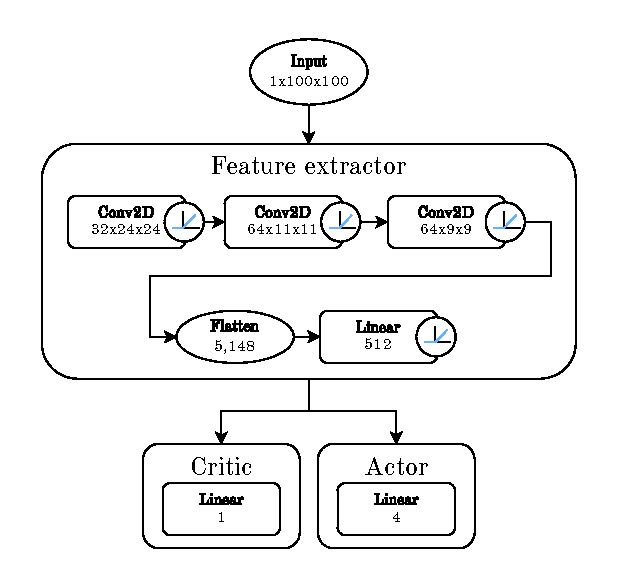
\includegraphics[width=1\linewidth]{diagrams/cnn_arch.pdf}
    \caption{Architecture used by SB3's \texttt{CnnPolicy}.}
    \label{fig:cnn_policy}
\end{figure}

\begin{figure}
    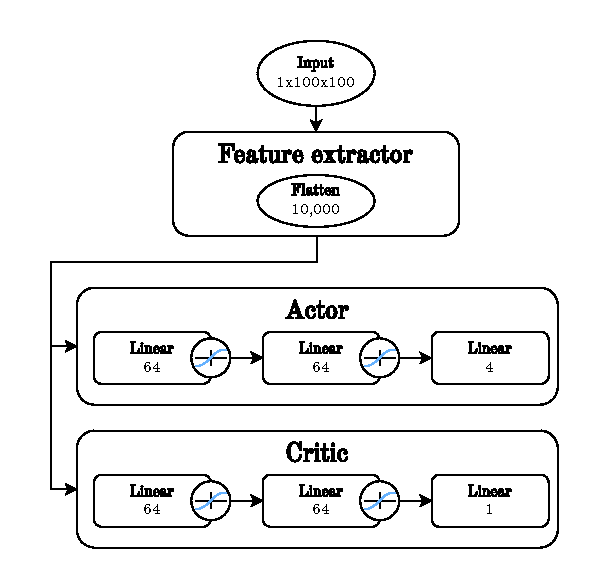
\includegraphics[width=1\linewidth]{diagrams/mlp_arch.pdf}
    \caption{Architecture used by SB3's \texttt{MlpPolicy}.}
    \label{fig:mlp_policy}
\end{figure}

\begin{figure}
    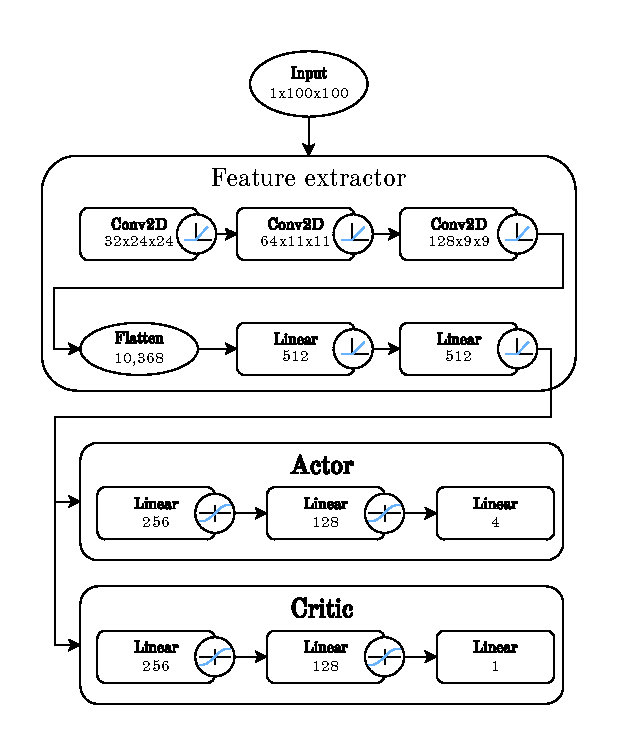
\includegraphics[width=1\linewidth]{diagrams/bigger_net_arch.pdf}
    \caption{Architecture of the network used in Subsection~\ref{subsec:arch_change}.}
    \label{fig:bigger_net_policy}
\end{figure}

\begin{figure}
    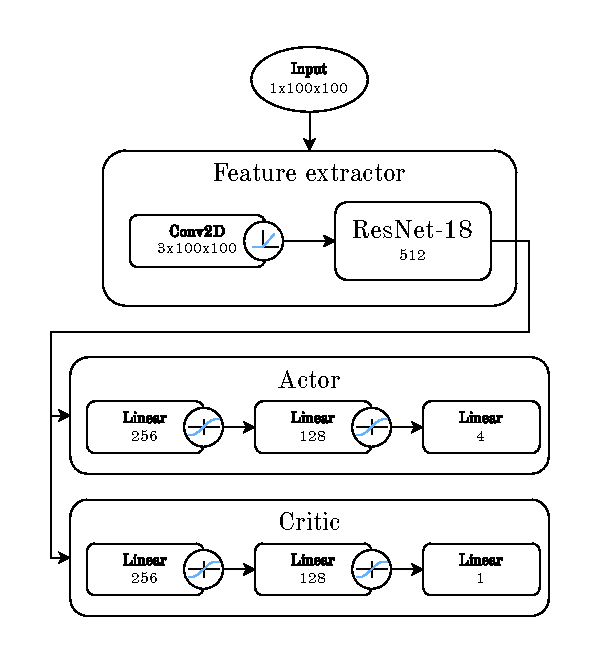
\includegraphics[width=1\linewidth]{diagrams/resnet_arch.pdf}
    \caption{Architecture of the network with a ResNet-18 feature extractor used in Subsection~\ref{subsec:resnet}.}
    \label{fig:resnet_arch}
\end{figure}

\begin{figure}
    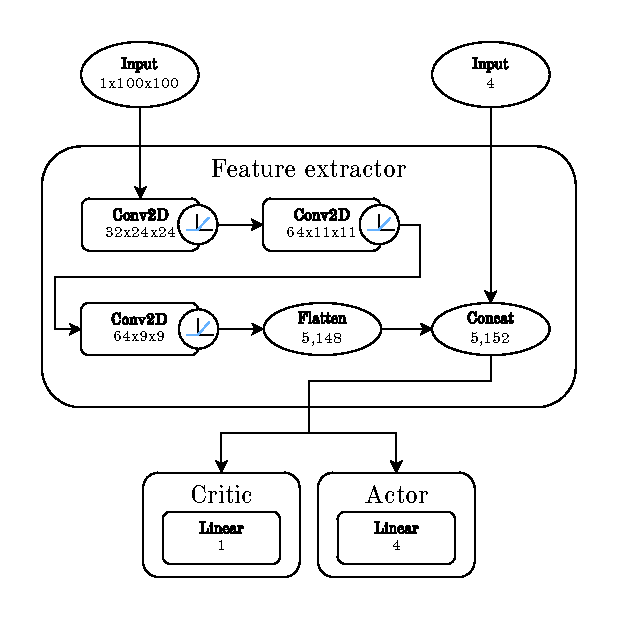
\includegraphics[width=1\linewidth]{diagrams/combined_policy.pdf}
    \caption{Architecture of the multi-input network introduced in Subsection~\ref{subsec:eval_metric}.}
    \label{fig:multiinput_arch}
\end{figure}

\begin{figure}
    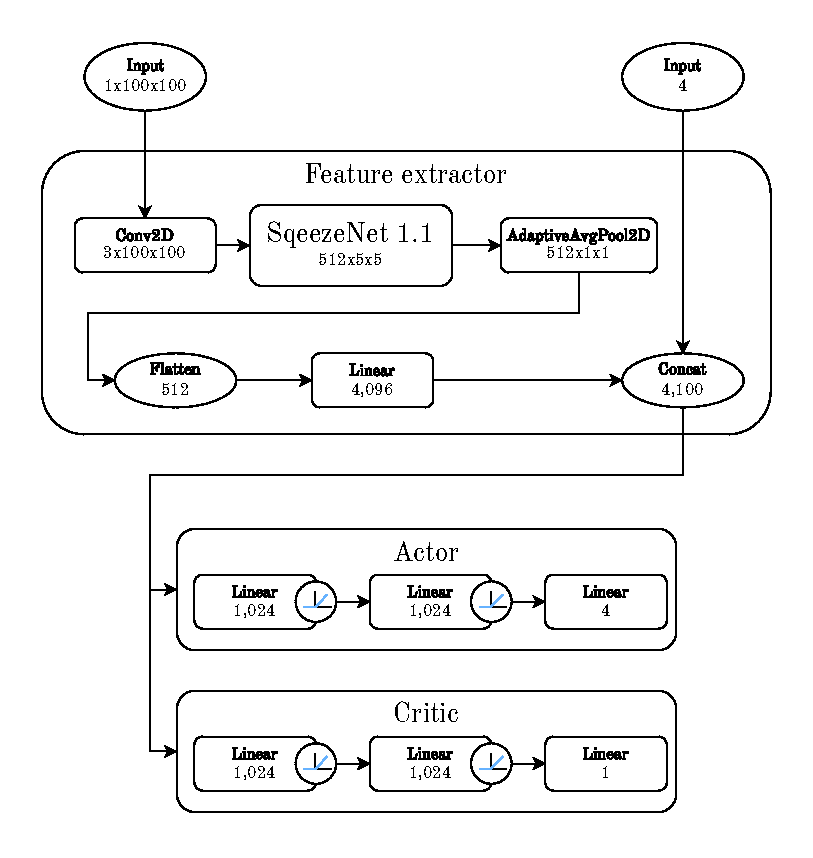
\includegraphics[width=1\linewidth]{diagrams/squeezenet.pdf}
    \caption{Architecture of the multi-input network with a SqueezeNet 1.1 feature extractor introduced in Subsection~\ref{subsec:feat_extract_two}.}
    \label{fig:squeezenet_arch}
\end{figure}

\chapter{CV detector algorithm}
\label{ap:cv}

This appendix describes in detail the algorithm used in the element detector based on traditional computer vision in Section~\ref{sec:trad_cv_detector}. The numerical parameter values mentioned in this section were tuned for images with a resolution of $1440\times900$ pixels. For images of a different size, some of them would have to be changed. Image processing is performed using the OpenCV library\footnote{\url{https://opencv.org/}}.

\section{Preprocessing}

The algorithm receives a screenshot of a website as input. The first step in the pipeline is preprocessing, which turns the colored image into a binary image that only contains relevant contours.

First, the image is converted from RGB to grayscale. This step is necessary because most image processing algorithms operate on single-channel images. Next, a bilateral filter is applied. Some websites use images or textures as backgrounds, which may be incorrectly detected as edges. The bilateral filter helps smooth these textures out while not destroying actual edges. This difference can be seen in Figure~\ref{fig:bilateral}. The parameters $d=21$, $\sigma_s =10$, and $\sigma_r = 50$ produced the most consistent results.

\begin{figure}
    \centering
    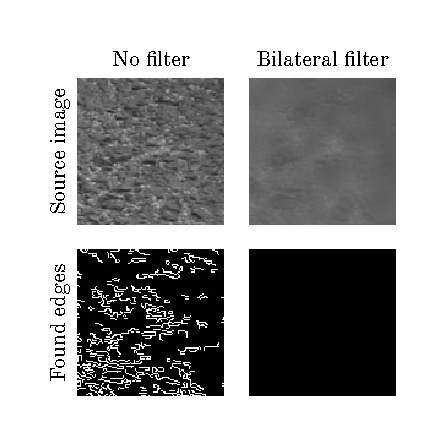
\includegraphics[width=1\linewidth]{diagrams/bilateral.pdf}
    \caption{Comparison of edges detected in an image of a road before and after a bilateral filter is applied. The original image comes from~\cite{aydos2020}.}
    \label{fig:bilateral}
\end{figure}

Next, Canny edge detection is used to find edge pixels. I chose Canny in particular since it already implements edge thinning and thresholding. Selecting appropriate thresholds posed challenges: low values increased noise detection, while high values risked omitting subtle features, such as text on a similarly colored background. I got the best results with $t_1=100$ and $t_2=200$.

A potentially more effective approach would involve applying the algorithm in multiple passes with varying thresholds. Filtering would be more strict with lower thresholds and less strict with higher thresholds. The results of these different passes would then be combined. However, as this implementation was intended as a prototype, and tuning the combinations of thresholds and filters would be time-intensive, this approach was not pursued.

Next, the edges are expanded using morphological dilation with a circular kernel. This addresses two issues. First, it compensates for incomplete or fragmented edge detection. Second, it merges letters of a text into a single blob. Distinguishing between textual contours and noise would be significantly more challenging without this step. This effect is shown in Figure~\ref{fig:dilation}.

\begin{figure}
    \centering
    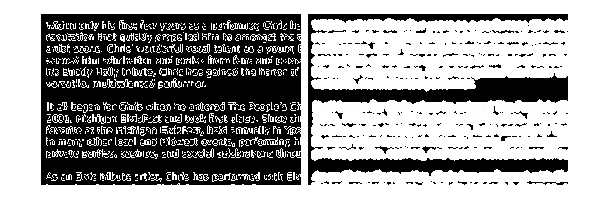
\includegraphics[width=1\linewidth]{diagrams/dilation.pdf}
    \caption{Text after edge detection before and after dilation. The original image comes from~\cite{aydos2020}.}
    \label{fig:dilation}
\end{figure}

Unfortunately, the dilation also sometimes joins together two separate elements. This issue is mitigated by removing one-pixel-wide connections (foreground pixels surrounded by foreground pixels in one direction but not in the other), though this solution is not perfect. Such pixels are detected using a hit-and-miss transformation and removed.

Following these preprocessing steps, the image can be processed for contour tracing. This is accomplished using OpenCV's implementation of the Suzuki–Abe algorithm.

\section{Contour filtering}

After preprocessing, the locations and coordinates of all contours in the image are available. I first reconstruct the hierarchy of these contours. Although OpenCV provides a contour hierarchy, it frequently contains errors. For example, a button with rounded corners frequently has gaps in its edges. As a result, text inside a button may be incorrectly identified as a sibling contour rather than a child.

To construct the tree, I first create a root contour that runs along the edge of the image and thus contains every other contour. I then sort the found contours in descending order based on the area of their axis-aligned bounding rectangle. Then, for each contour, I check whether its bounding rectangle is mostly within any of the root node's children, in which case I check through its children and repeat recursively. If not, it becomes a new child of the checked node.

The next step is contour filtering. A contour is eliminated if at least one of the following is true. The filtering results are visible in Figure~\ref{fig:filtering}. These rules were developed by analyzing false element predictions and identifying which attributes distinguished them from valid elements.

\begin{enumerate}
    \item Its bounding rectangle is too small (height or width less than 15 pixels, or both dimensions under 30 pixels).
    \item Its parent is too small (only contours of at least $100 \times 100$ pixels may have children).
    \item It is excessively rotated (i.e., the minimum-area enclosing rectangle is rotated by more than 10 degrees). This rule is not applied to contours with an approximately square aspect ratio.
    \item It is at least slightly rotated, and the area of its convex hull is notably smaller than that of its bounding rectangle (less than 75 percent).
    \item It is an inside contour (it encloses only background pixels).
\end{enumerate}

\begin{figure}
    \centering
    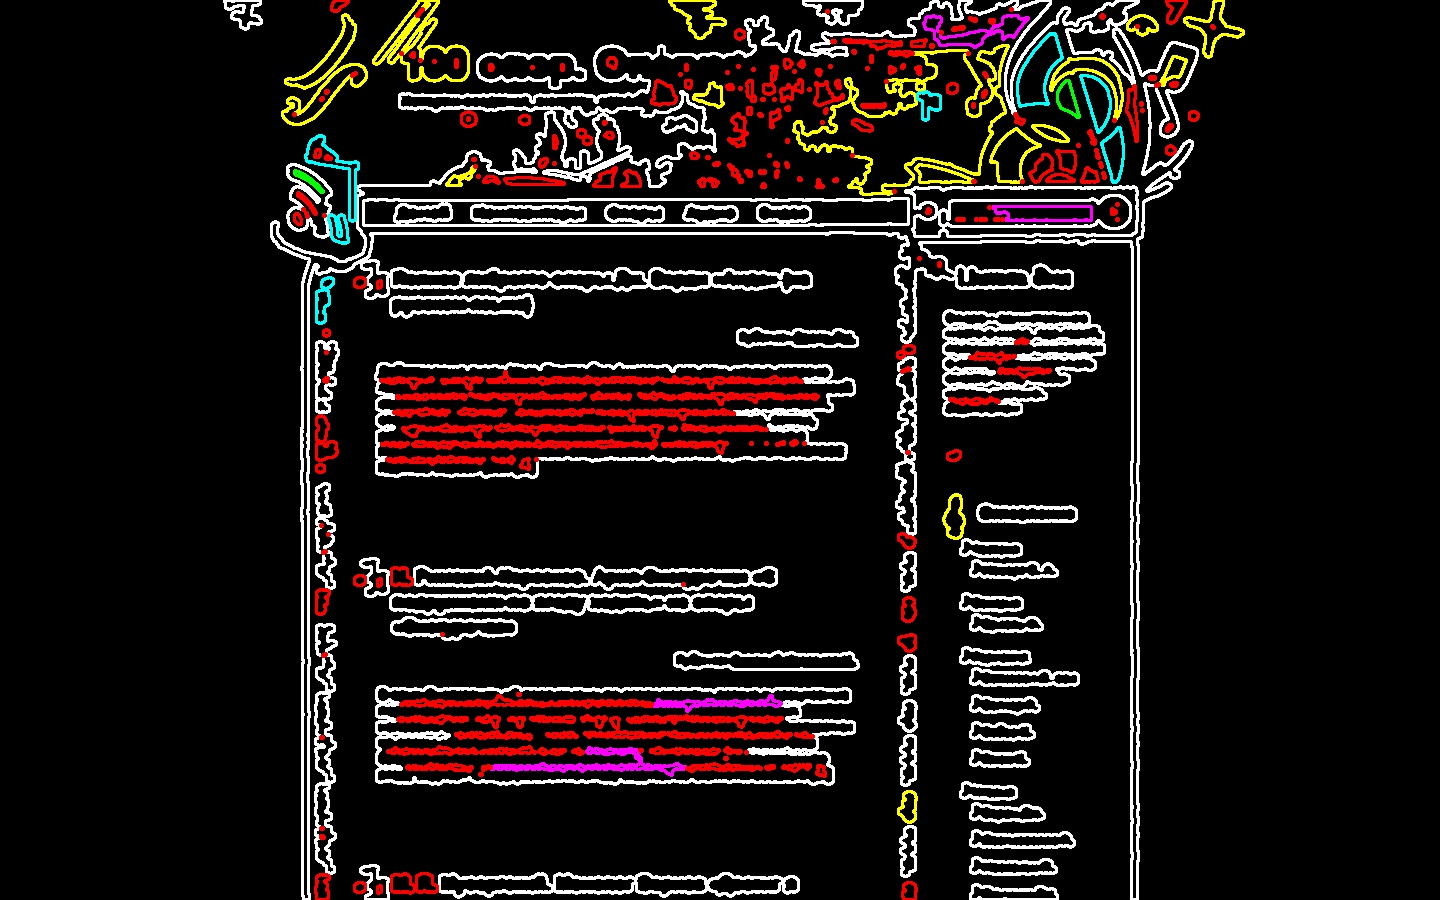
\includegraphics[width=1\linewidth]{diagrams/filter.jpg}
    \caption{The image shows the contour filtering. White contours survived, red contours were too small, green contours' parents were too small, light blue contours were too rotated, yellow contours had a small convex hull, and magenta contours were inside contours. The original image comes from~\cite{aydos2020}.}
    \label{fig:filtering}
\end{figure}

Finally, any two contours whose bounding rectangles intersect, without one being fully contained within the other, are merged. The axis-aligned bounding boxes of the filtered and merged contours constitute the final output of the algorithm.

The most challenging element types for this implementation were text and raster images. Unlike other elements, text consists of many small contours corresponding to individual letters rather than a single contiguous region. Distinguishing between contours representing letters and those resulting from random noise can be difficult.

Raster images are problematic due to the presence of numerous irregular and irrelevant edges that do not correspond to meaningful elements. This issue is particularly difficult to address when background images introduce edges that overlap or interfere with those of genuine UI elements.

\chapter{List of digital appendices}

\begin{enumerate}
    \item \texttt{WebElementDetector.zip} -- An archive containing the implementations of the environments, the CV-based detector, and scripts for training, evaluating, benchmarking, and running all the detectors.
    \item \texttt{Models.zip} -- An archive containing the best RL and YOLO models trained on the three sizes of datasets.
\end{enumerate}

\end{document}
